% -*- coding: utf-8 -*-
\documentclass[UTF8,a4paper,10pt,fontset=fandol]{ctexart}

\usepackage[left=3.0cm, right=3.0cm, top=2.6cm, bottom=2.6cm]{geometry}
\usepackage{amsmath}
\usepackage{graphicx}
\usepackage{float}
\usepackage{caption}
\usepackage{booktabs}
\usepackage{multirow}
\usepackage{tabularx}
\usepackage{array}
\usepackage{longtable}
\usepackage{enumitem}
\usepackage{hyperref}
\usepackage{fancyhdr}
\usepackage[table]{xcolor}

\newcommand{\yihao}{\fontsize{26pt}{36pt}\selectfont}
\newcommand{\erhao}{\fontsize{22pt}{28pt}\selectfont}
\newcommand{\xiaoer}{\fontsize{18pt}{18pt}\selectfont}
\newcommand{\sanhao}{\fontsize{16pt}{24pt}\selectfont}
\newcommand{\sihao}{\fontsize{14pt}{21pt}\selectfont}
\newcommand{\xiaosi}{\fontsize{12pt}{18pt}\selectfont}
\newcommand{\wuhao}{\fontsize{10.5pt}{15.75pt}\selectfont}
\newcolumntype{Y}{>{\raggedright\arraybackslash}X}

\ctexset{
    section = {name = {,、}, number = \chinese{section}},
    subsection = {name = {（,）}, number = \chinese{subsection}}
}

\pagestyle{fancy}
\raggedbottom
\lhead{\kaishu \leftmark}
\rhead{\kaishu 软件设计报告}
\lfoot{}
\cfoot{\thepage}
\rfoot{}
\renewcommand{\headrulewidth}{0.1pt}
\renewcommand{\footrulewidth}{0pt}
\newcommand{\HRule}{\rule{\linewidth}{0.5mm}}

\hypersetup{
    colorlinks=true,
    linkcolor=black,
    urlcolor=blue
}

\setlist[itemize]{nosep,leftmargin=2em}
\setlist[enumerate]{nosep,leftmargin=2.2em}
\captionsetup[figure]{font=small}

\begin{document}

\begin{titlepage}
    \begin{center}
        
\includegraphics[width=0.8\textwidth]{NKU.png}\\[1cm]
        \textsf{\Huge \kaishu{\textbf{南\ \ \ \ \ \ 开\ \ \ \ \ \ 大\ \ \ \ \ \ 学}} }\\[0.9cm]
        \textsf{\huge \kaishu{\textbf{计\ \ 算\ \ 机\ \ 学\ \ 院}}}\\[0.5cm]
        \textsf{\Large \textbf{软件工程实验报告}}\\[0.8cm]
        \HRule \\[0.9cm]
        {\LARGE \bfseries 智能城市生成系统软件设计报告}\\[0.4cm]
        \HRule \\[2.0cm]
        \textsf{\LARGE 林晖鹏}\\[0.5cm]
        \textsf{\LARGE \kaishu{年级\ :\ 2023级}}\\[0.5cm]
        \textsf{\LARGE \kaishu{专业\ :\ 计算机科学与技术}}\\[0.5cm]
        \textsf{\LARGE \kaishu{指导教师\ :\ 李起成}}\\[0.5cm]
        \vfill
        {\Large \today}
    \end{center}
\end{titlepage}

\newpage
% \thispagestyle{empty}
% \renewcommand{\abstractname}{\kaishu \sihao \textbf{摘要}}
% \begin{abstract}
% 本文面向课程作业“智能城市生成系统软件设计”，在前期需求分析基础上，进一步给出系统的软件设计说明。报告参考软件设计说明文档（Software Design Description, SDD）的组织方式，围绕系统概述、架构设计、数据设计、面向对象设计和界面设计展开，重点说明主系统、Blender 插件执行端、资产与项目数据层、动态仿真模块以及大语言模型解析服务之间的职责划分与协作关系。

% 相较于需求分析阶段，本报告更加关注“系统如何被组织起来”。一方面，报告从模块视角解释用户工作台、任务调度、插件适配、LLM 解析、资源管理、仿真分析等子系统如何协同；另一方面，报告从对象视角归纳项目、场景、任务、资产、草图、布局、仿真对象与日志等核心实体，并为后续类图、顺序图、状态图和部署图的绘制提供统一语义基础。对于课程要求中的八类 UML 图，本文在面向对象设计章节中给出图的设计目标、建议表达重点与建模边界，便于后续逐步补齐正式图件。

% 本报告的设计原则包括：以角色分工驱动界面组织，以任务流驱动模块协作，以结构化任务驱动 Blender 执行，以版本化数据支撑回溯与比较，以可解释与可确认机制约束 LLM 解析结果。通过这些设计，系统既保留程序化建模的执行确定性，又引入自然语言与多模态交互带来的表达便利性。

% \noindent \textbf{关键词：}软件设计；SDD；UML；Blender；智能城市生成系统；大语言模型
% \end{abstract}

\tableofcontents
\newpage

\section{引言}

\subsection{编写目的}
本文档用于说明智能城市生成系统的软件设计方案，其目标读者包括课程指导教师、项目成员以及后续补充 UML 图和实现代码的开发者。与需求分析报告相比，本报告不再重点讨论“系统需要做什么”，而是重点回答“系统如何组织起来实现这些需求”。因此，文档需要为后续概要实现、模块拆分、类关系细化、接口对接和图件绘制提供统一设计依据。

\subsection{项目范围}
智能城市生成系统面向三维城市场景快速生成、布局调整、资产替换、生态塑造、动态仿真和智能交互等任务，服务对象包括场景建模师、行业分析师和系统管理员三类角色。系统以 Blender 作为三维执行环境，以主系统作为任务组织与展示入口，并通过资产库、项目库、日志库和大语言模型服务形成完整的设计闭环。

\subsection{文档结构}
本报告共分为七个部分。第一部分为引言，说明文档目的与范围；第二部分给出系统概述；第三部分描述系统架构及模块分解；第四部分说明核心数据设计；第五部分从面向对象角度组织八类 UML 图；第六部分说明界面设计；第七部分给出总结。这样的结构基本对应课程提供的 SDD 模板，同时保留了本项目“任务流驱动 + 插件执行 + LLM 解析”的系统特征。

\subsection{参考资料}
\begin{enumerate}[label=\arabic*.]
    \item IEEE 1016-2009, \textit{IEEE Standard for Information Technology--Systems Design--Software Design Descriptions}. 可参考：\url{https://standards.ieee.org/standard/1016-2009.html}
    \item ISO/IEC/IEEE 42010:2022, \textit{Software, systems and enterprise --- Architecture description}. 可参考：\url{https://www.iso.org/standard/74393.html}
    \item Object Management Group (OMG), \textit{Unified Modeling Language (UML), Version 2.5.1}. 可参考：\url{https://www.omg.org/spec/UML}
    \item Blender Python API Overview. 官方文档：\url{https://docs.blender.org/api/current/info_overview.html}
    \item Blender Add-on Tutorial. 官方文档：\url{https://docs.blender.org/manual/en/latest/advanced/scripting/addon_tutorial.html}
    \item 第二次个人作业《智能城市生成系统需求分析报告》，作为本报告的软件需求与功能边界来源。
\end{enumerate}

\subsection{术语与缩略语}
\begin{table}[H]
\centering
\caption{术语说明表}
\rowcolors{2}{gray!8}{white}
\begin{tabularx}{\textwidth}{p{3cm} Y}
\rowcolor{gray!20}
\toprule
术语 & 含义说明 \\
\midrule
主系统 & 面向用户的控制平台，负责登录、任务组织、结果展示和后台治理 \\
Blender 插件 & 在 Blender 中执行建模、替换、布局更新和场景保存任务的插件组件 \\
结构化任务 & 由对象、属性、数量、空间关系、目标区域和执行参数构成的统一任务表示 \\
资产库 & 存储道路、建筑、树木、庭院、水体、山体和动态对象资源的信息集合 \\
场景版本 & 某一项目在一次生成或修改完成后的可回溯状态快照 \\
LLM & Large Language Model，大语言模型，用于自然语言和多模态输入解析 \\
仿真模块 & 为车辆、人群、船只等对象生成动态展示效果的子系统 \\
SDD & Software Design Description，软件设计说明文档 \\
\bottomrule
\end{tabularx}
\end{table}

\section{系统概述}
\label{sec:system_overview}

\subsection{系统目标}
智能城市生成系统的设计目标不是单纯提供一个建模界面，而是构建一个能够支撑“意图输入 - 任务转换 - 三维执行 - 结果反馈 - 版本沉淀”的软件系统。结合课程主题，系统需要同时满足以下目标：
\begin{enumerate}[label=\arabic*.]
    \item 面向建模师提供高效率的基础场景生成与局部修改能力。
    \item 面向分析师提供清晰的结果查看、仿真比较与导出能力。
    \item 面向管理员提供权限、资源、模型服务与日志治理能力。
    \item 通过结构化任务机制连接上层交互和底层 Blender 执行。
    \item 通过 LLM 降低表达门槛，但保留确认、纠错和回退能力。
\end{enumerate}

\subsection{用户视角概述}
系统的三类核心角色分别具有不同的使用重心。场景建模师关注生成效率、参数控制和多轮修改；行业分析师关注展示效果、方案比较和导出结果；系统管理员关注权限隔离、资源状态、服务可用性与审计追踪。因此，系统在设计上不能把三类用户混成统一入口下的同质操作流，而应围绕角色工作台进行组织。

\begin{figure}[t]
\centering

\includegraphics[width=\textwidth]{figures/1.png}
\caption{系统整体业务概览}
\label{fig:system_overview}
\end{figure}

\subsection{核心设计思想}
本系统的软件设计遵循以下几项核心思想。
\begin{enumerate}[label=\arabic*.]
    \item 角色驱动：先按角色划分工作台，再在工作台内部组织操作链路。
    \item 任务驱动：所有核心能力最终都归约为可跟踪的任务，而不是零散按钮操作。
    \item 执行解耦：主系统负责理解和编排，Blender 插件负责几何与场景执行。
    \item 数据留痕：项目、场景、任务、日志和解析结果都需要保留版本和过程信息。
    \item 智能受控：LLM 负责辅助理解，不直接越过确认机制修改场景。
\end{enumerate}

\subsection{运行上下文}
从运行形态上看，智能城市生成系统由五类要素共同组成：用户界面层、任务组织层、三维执行层、数据资源层和智能解析层。用户通过主系统表达设计意图；主系统将输入转换为结构化任务；Blender 插件依据任务完成场景生成与修改；资产库、项目库和日志库负责支撑数据持久化；LLM 服务提供自然语言与多模态输入的解释能力；仿真模块在执行结果基础上补充动态表现。

\section{系统架构}
\label{sec:system_architecture}

\subsection{总体架构设计}
系统采用“主系统 + 插件执行端 + 数据资源层 + 智能解析服务 + 仿真分析模块”的分层协作结构。这样设计的原因在于：用户交互、任务理解、三维执行、数据存储和动态展示的变化频率并不一致，将它们拆开能够减少耦合，并方便后续单独扩展模型服务、插件能力或资源类型。

\begin{table}[t]
\centering
\caption{高层子系统职责划分}
\label{tab:subsystem_responsibilities}
\rowcolors{2}{gray!8}{white}
\begin{tabularx}{\textwidth}{p{3.2cm} Y}
\rowcolor{gray!20}
\toprule
子系统 & 核心职责 \\
\midrule
用户工作台 & 提供登录、项目浏览、参数配置、任务确认、结果查看和导出交互 \\
任务调度 & 接收输入、校验权限、封装任务、分发执行、跟踪状态与回写结果 \\
LLM 解析 & 将自然语言、草图摘要和上下文解析为结构化任务建议 \\
Blender 插件适配 & 接收结构化任务并完成建模、替换、布局更新和场景保存 \\
资源与项目数据 & 保存项目、场景、资产、布局数据、任务记录与日志数据 \\
动态仿真 & 在生成后的场景上配置车辆、人群和船只等动态展示效果 \\
后台治理 & 管理用户、角色、权限、插件状态、模型服务和审计日志 \\
\bottomrule
\end{tabularx}
\end{table}

\subsection{分层关系说明}
\begin{enumerate}[label=\arabic*.]
    \item 表现层：由建模师工作台、分析师工作台和管理员工作台组成，负责输入和展示。
    \item 应用层：由任务调度、项目管理、版本管理、权限控制等服务组成，负责流程编排。
    \item 领域层：由场景、布局、任务、资产、仿真和日志等核心领域对象组成，负责表达业务语义。
    \item 基础设施层：由 Blender 插件接口、数据库、文件存储、模型服务接口组成，负责外部依赖接入。
\end{enumerate}

\subsection{模块分解说明}
\subsubsection*{1. 系统整体结构分解}

图~\ref{fig:system_overview}描述了系统在高层视角下的整体结构。系统首先划分为统一登录与身份认证入口，以及面向不同角色的三个工作台：场景建模师工作台、行业分析师工作台和系统管理员工作台。建模师工作台负责场景创建、布局调整、插件调用和结果修订；分析师工作台负责场景查看、动态仿真、方案比较与结果导出；管理员工作台负责用户管理、权限配置、模型服务维护和日志审计。

在角色工作台之外，系统还进一步分解出结果与治理相关的公共支撑部分，包括项目结果管理、版本留存和日志记录。三个工作台在完成各自任务后，均需要与这些公共支撑部分发生交互，以保证系统具备结果保存、版本回溯和行为追踪能力。由此形成的高层结构说明，本系统不是单一建模工具，而是由统一入口、角色工作台和公共支撑模块共同组成的协同系统。

\subsubsection*{2. 系统数据与任务流分解}
\begin{figure}[H]
\centering
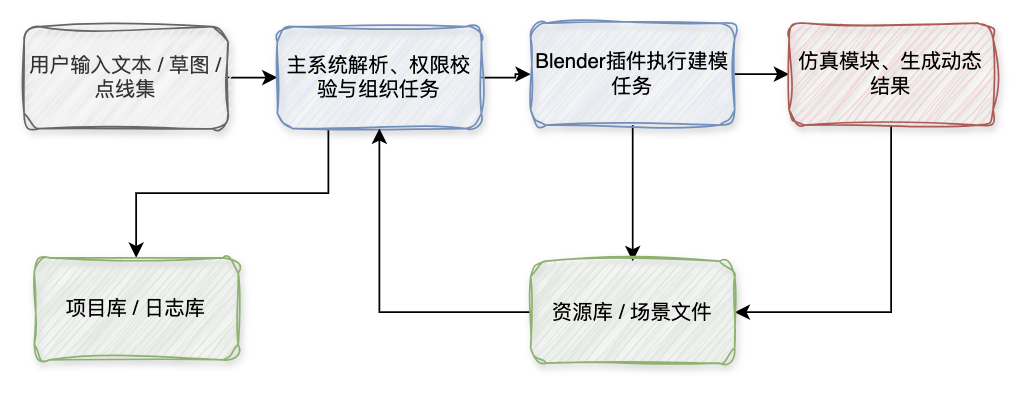
\includegraphics[width=\textwidth]{figures/8.png}
\caption{系统数据与任务流分解图}
\label{fig:architecture_data_flow}
\end{figure}

图~\ref{fig:architecture_data_flow}反映了系统在执行链路上的组成方式。按照任务流和数据流关系，系统可分解为主系统、Blender 插件、资产库、场景文件、仿真模块、项目库和日志库。主系统负责接收用户输入并完成权限判断、输入规范化、参数补全和任务封装；Blender 插件负责执行具体生成与修改任务；资产库和场景文件为插件执行提供资源与场景上下文；仿真模块负责在生成结果基础上补充动态展示；项目库和日志库分别负责结果版本保存与执行过程留痕。

这些部分之间通过统一任务链路衔接：输入先进入主系统，任务由主系统下发至 Blender 插件，执行结果回流至主系统并同步写入项目库和日志库，涉及动态对象时再继续流入仿真模块。由此形成的分解结果明确了各子系统在执行链路中的职责边界，也明确了任务、结果和日志在系统中的回写路径。

\subsubsection*{3. 系统功能结构分解}
\begin{figure}[H]
\centering
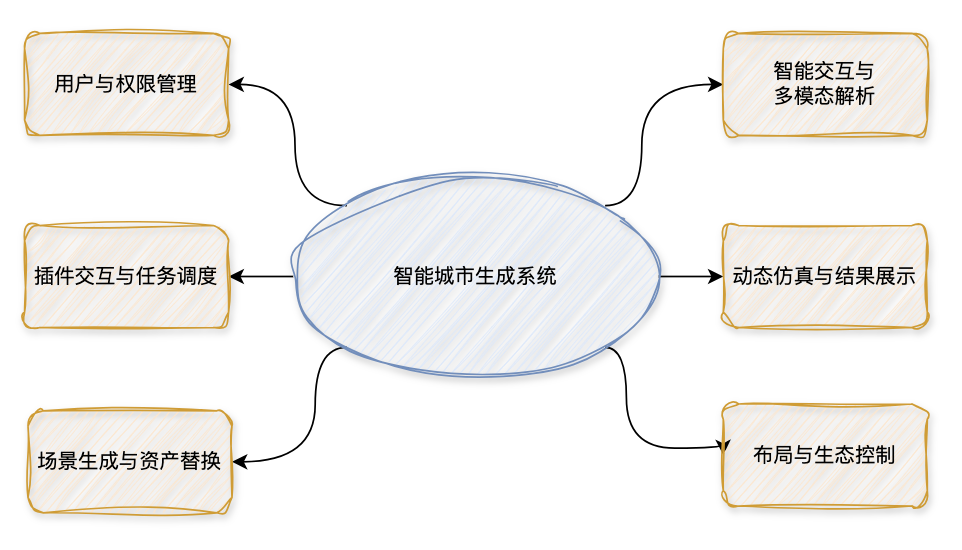
\includegraphics[width=\textwidth]{figures/9.png}
\caption{系统功能结构分解图}
\label{fig:function_structure}
\end{figure}

图~\ref{fig:function_structure}从功能视角展示了系统的模块划分。根据需求边界与职责划分，系统功能可分解为六个核心模块：用户与权限管理、插件交互与任务调度、场景生成与资产替换、布局与生态控制、智能交互与多模态解析、动态仿真与结果展示。其中，用户与权限管理负责系统入口控制与后台治理；插件交互与任务调度负责连接主系统与 Blender 执行端；场景生成与资产替换负责基础城市场景构建与对象替换；布局与生态控制负责空间结构调整与生态对象生成；智能交互与多模态解析负责自然语言、草图和参数表单的统一理解；动态仿真与结果展示负责车辆、人群、船只等动态效果呈现与结果导出。

在此基础上，各模块之间形成清晰的协作关系：权限模块提供访问边界，任务调度模块组织执行链路，场景生成与布局控制模块承担主要建模能力，智能交互模块负责把用户意图转化为可执行任务，动态仿真模块负责补充结果展示。这样的分解结果使系统后续能够围绕模块边界开展接口定义、对象划分和实现分工。

\subsection{架构决策说明}
\begin{enumerate}[label=\arabic*.]
    \item 不让 LLM 直接操作 Blender，而是先生成结构化任务，以保证执行可控。
    \item 不让场景结果只保留最终态，而是保留项目和场景版本，支撑回滚与比较。
    \item 不将仿真逻辑与基础建模强耦合，便于只做静态生成或后续升级动态能力。
    \item 不让管理员直接介入建模链路，而是通过治理模块进行用户、资源和服务维护。
\end{enumerate}

\section{数据设计}
\label{sec:data_design}

\subsection{数据描述}
系统的数据设计需要同时服务三种目标：支持任务执行、支持结果回溯、支持系统治理。因此，数据不应只按“表存什么”理解，而应按“哪些对象支撑哪些设计行为”理解。结合前期需求分析，本系统的核心数据可以归纳为以下几类：
\begin{enumerate}[label=\arabic*.]
    \item 用户与权限数据：支撑角色识别、权限控制和菜单装载。
    \item 项目与场景数据：支撑项目管理、版本回溯和结果比较。
    \item 资产与资源数据：支撑生成、替换和风格联动。
    \item 布局与草图数据：支撑精确布局和草图驱动的空间调整。
    \item 任务与解析数据：支撑 LLM 理解、结构化任务生成和执行跟踪。
    \item 仿真与展示数据：支撑车辆、人群、船只等动态展示能力。
    \item 日志与审计数据：支撑故障定位、责任追踪和后台治理。
\end{enumerate}

从存储组织方式看，系统数据并不全部采用同一种结构保存。用户、角色、项目、任务状态和日志记录等信息适合采用结构化存储，以保证查询、过滤和审计效率；场景版本、布局结果、结构化任务内容和仿真配置等信息更适合采用半结构化存储，以保留复杂对象关系和可扩展字段；草图图像、场景文件和资源文件则以文件形式保存，并通过项目编号、场景版本编号或任务编号与结构化记录建立关联。这样的组织方式既能满足管理型数据的一致性要求，也能兼顾三维场景系统中复杂对象与外部文件共存的特点。

在数据转换路径上，系统首先将用户输入转化为可管理的数据对象，再根据对象类型进入不同处理链路。参数表单输入会直接形成结构化配置记录，草图和点线集会形成布局数据与中间识别结果，自然语言和多模态输入会形成解析记录与结构化任务，最终再与场景版本、仿真配置和日志记录建立关联。通过这一转换方式，系统能够将需求表达、任务执行和结果输出统一纳入可追踪的数据体系之中。

\subsection{数据流说明}
\begin{figure}[H]
\centering
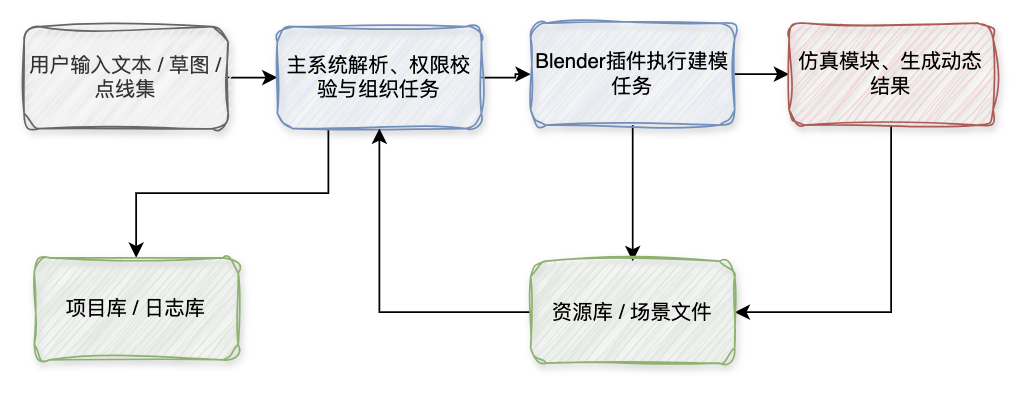
\includegraphics[width=\textwidth]{figures/8.png}
\caption{系统数据流图}
\label{fig:data_flow}
\end{figure}

从数据流角度看，用户输入先进入主系统进行规范化处理；之后输入被封装为任务并交给插件或 LLM 服务；执行结果回写场景和版本数据；仿真结果作为附加展示结果保存；关键过程同步写入日志。这样的设计可以将“输入、理解、执行、展示、审计”五个环节通过统一任务标识串联起来。

\subsection{核心实体设计}
\subsubsection*{1. 核心实体分组}
根据系统职责边界，核心实体可划分为五组。第一组为身份与权限实体，包括 \texttt{User}、\texttt{Role} 和权限相关记录，用于描述用户身份、访问边界和菜单装载规则；第二组为项目与场景实体，包括 \texttt{Project} 和 \texttt{SceneVersion}，用于描述项目生命周期以及多轮生成后的场景快照；第三组为资源与布局实体，包括 \texttt{Asset}、\texttt{LayoutSet} 和 \texttt{SketchImage}，用于表达生成所依赖的资源、空间控制信息和原始设计输入；第四组为任务与解析实体，包括 \texttt{Task} 和 \texttt{StructuredCommand}，用于连接用户意图、LLM 解析结果和插件执行过程；第五组为仿真与审计实体，包括 \texttt{SimulationPlan} 和 \texttt{OperationLog}，用于支撑动态展示与系统维护。

上述分组方式的目的，是将管理型对象、业务型对象和过程型对象区分开来。这样处理后，系统在实现时可以分别围绕用户治理、项目版本管理、场景执行链路和日志审计链路设计数据表、文件组织方式与接口输入输出格式，避免把所有数据混杂在同一层面中。

\subsubsection*{2. 核心实体与职责}
\begin{table}[H]
\centering
\caption{核心实体与职责}
\label{tab:core_entities}
\rowcolors{2}{gray!8}{white}
\begin{tabularx}{\textwidth}{p{2.2cm} p{1.8cm} p{2.2cm} Y}
\rowcolor{gray!20}
\toprule
实体 & 类型 & 主要存储形态 & 设计职责 \\
\midrule
User & 结构化实体 & 数据表/结构化记录 & 表示系统用户身份、账号状态与角色归属。 \\
Role & 结构化实体 & 数据表/结构化记录 & 表示角色类别及其对应权限集合。 \\
Project & 结构化实体 & 数据表/结构化记录 & 组织一个城市场景设计任务的生命周期。 \\
SceneVersion & 半结构化实体 & 结构化记录 + 场景文件关联 & 保存某次生成或修改后的场景状态快照。 \\
Asset & 半结构化实体 & 资源元数据 + 文件路径 & 记录资源类别、标签、路径、版本和适用条件。 \\
LayoutSet & 半结构化实体 & JSON/对象记录 & 描述点、线、面和控制参数构成的布局结果。 \\
SketchImage & 文件实体 & 图像文件 + 关联记录 & 保存用户上传草图及其识别关联信息。 \\
Task & 结构化实体 & 数据表/结构化记录 & 表示统一的可跟踪执行任务。 \\
StructuredCommand & 半结构化实体 & JSON/对象记录 & 表示解析后的对象、属性、关系与参数建议。 \\
SimulationPlan & 半结构化实体 & JSON/对象记录 & 保存动态对象配置与仿真参数。 \\
OperationLog & 结构化实体 & 日志表/结构化记录 & 保存关键操作、状态与异常信息。 \\
\bottomrule
\end{tabularx}
\end{table}

\subsubsection*{3. 实体关系说明}
核心实体之间存在较为明确的关联关系。一个 \texttt{User} 对应一个角色集合或角色标识，并以该角色参与项目创建、任务提交和后台管理等行为；一个 \texttt{Project} 可以关联多个 \texttt{SceneVersion}，用于记录同一项目在不同时间点的生成与修改结果；一个 \texttt{Task} 通常关联一次结构化任务内容、一次执行状态演化过程以及若干日志记录；一个 \texttt{SceneVersion} 可以引用多个 \texttt{Asset} 和一个或多个 \texttt{LayoutSet}，从而说明该版本场景由哪些资源和空间结构共同构成；当任务涉及动态展示时，还会进一步关联 \texttt{SimulationPlan}。

这种实体关系设计保证了系统能够回答几个关键问题：某个场景版本是由谁在什么项目中生成的、它依赖了哪些资源、它对应了哪次任务、任务经历了哪些状态变化、是否产生了动态仿真结果、出现异常时又应追溯到哪条日志记录。对软件设计而言，这些关系比单个字段本身更重要，因为它们决定了后续接口设计、数据库设计和对象建模时的主关联路径。

\subsection{数据字典}
{
\renewcommand{\arraystretch}{1.3}
\rowcolors{3}{gray!8}{white}
\begin{longtable}{p{2.5cm} p{1.8cm} p{2.0cm} p{6.0cm}}
\caption{主要数据字典}\label{tab:sdd_data_dict}\\
\toprule
\rowcolor{gray!20}
\textbf{数据项} & \textbf{类型} & \textbf{来源} & \textbf{说明} \\
\midrule
\endfirsthead
\toprule
\rowcolor{gray!20}
\textbf{数据项} & \textbf{类型} & \textbf{来源} & \textbf{说明} \\
\midrule
\endhead
\midrule
\multicolumn{4}{r}{\small 续下页}\\
\endfoot
\bottomrule
\endlastfoot
\texttt{user\_id} & 字符串 & 用户管理 & 用户唯一标识。 \\
\texttt{role\_type} & 枚举 & 权限模块 & 取值可为建模师、分析师、管理员。 \\
\texttt{project\_id} & 字符串 & 项目模块 & 项目唯一标识，用于组织场景与任务。 \\
\texttt{scene\_version\_id} & 字符串 & 场景模块 & 场景某次保存结果的唯一编号。 \\
\texttt{asset\_id} & 字符串 & 资产库 & 资产唯一标识，关联类别和资源路径。 \\
\texttt{layout\_payload} & JSON/对象 & 布局模块 & 保存道路、边界、区域等几何描述。 \\
\texttt{sketch\_path} & 文件路径 & 上传模块 & 草图文件位置，用于识别与追溯。 \\
\texttt{task\_id} & 字符串 & 调度模块 & 用于串联解析、执行、日志与结果。 \\
\texttt{task\_status} & 枚举 & 调度模块 & 典型状态包括待确认、排队中、执行中、成功、失败。 \\
\texttt{command\_spec} & JSON/对象 & LLM 模块 & 保存对象、属性、数量和空间关系等结构化结果。 \\
\texttt{sim\_config} & JSON/对象 & 仿真模块 & 保存动态对象数量、路径与速度等参数。 \\
\texttt{log\_message} & 文本 & 日志模块 & 保存关键操作或异常信息。 \\
\end{longtable}
}

\subsection{数据设计原则}
\begin{enumerate}[label=\arabic*.]
    \item 统一标识原则：项目、场景、任务和日志之间通过唯一编号建立关联。
    \item 版本保留原则：场景修改不直接覆盖，重要结果应沉淀为可回看版本。
    \item 过程可解释原则：LLM 解析结果要保留中间结构，而不仅是最终执行结果。
    \item 资源可管理原则：资产需要有类别、标签、版本和适用范围，便于筛选与治理。
\end{enumerate}

\section{面向对象设计}

\subsection{设计说明}
面向对象设计部分从参与者边界、核心对象、活动控制、交互时序、对象协作、状态演化、软件构成和运行部署八个层面描述系统。各类图围绕同一组核心概念展开，包括场景建模师、行业分析师、系统管理员、项目、场景版本、任务、结构化命令、插件作业、执行结果以及日志与仿真对象。通过统一角色命名、任务边界和结果承接对象，不同图件能够共同刻画系统从输入到执行、从结果生成到版本留存的完整设计。

\subsection{用例图}
图\ref{fig:oo_usecase} 展示了系统对外提供的主要能力及其角色边界。场景建模师通过登录认证进入建模工作区，可执行项目管理、场景建模、布局调整、智能修改和结果导出等操作；行业分析师进入分析工作区后执行结果分析与结果导出；系统管理员进入治理工作区后执行权限配置、日志审计和服务监控。图中还明确了智能修改与草图解析、任务确认、插件执行之间的包含关系，以及结果分析与结果导出之间的扩展关系。

从功能划分上看，建模工作区对应系统的生产链路，分析工作区对应系统的结果消费链路，治理工作区对应系统的运行维护链路，三者以登录认证作为统一入口，并在系统边界内形成相互独立但共享数据成果的能力分区。场景建模师能够直接触发场景生成、布局调整和智能修改，因此其用例最靠近任务执行与场景版本生成；行业分析师不直接参与生成，而是建立在既有版本和仿真结果之上完成观察、比较和导出；系统管理员则不处理具体业务结果，而是保障权限、服务和审计环境的稳定运行。

该图在设计层面说明了两个关键问题。其一，系统采用按角色分区、按工作台组织能力的外部交互方式，不同角色的可见能力集合并不相同。其二，智能修改并不是孤立能力，而是以内含的草图解析、任务确认和插件执行为处理链路，因此其实现上必然关联自然语言解析、约束检查和插件调度三个内部机制。

\begin{figure}[!htbp]
\centering
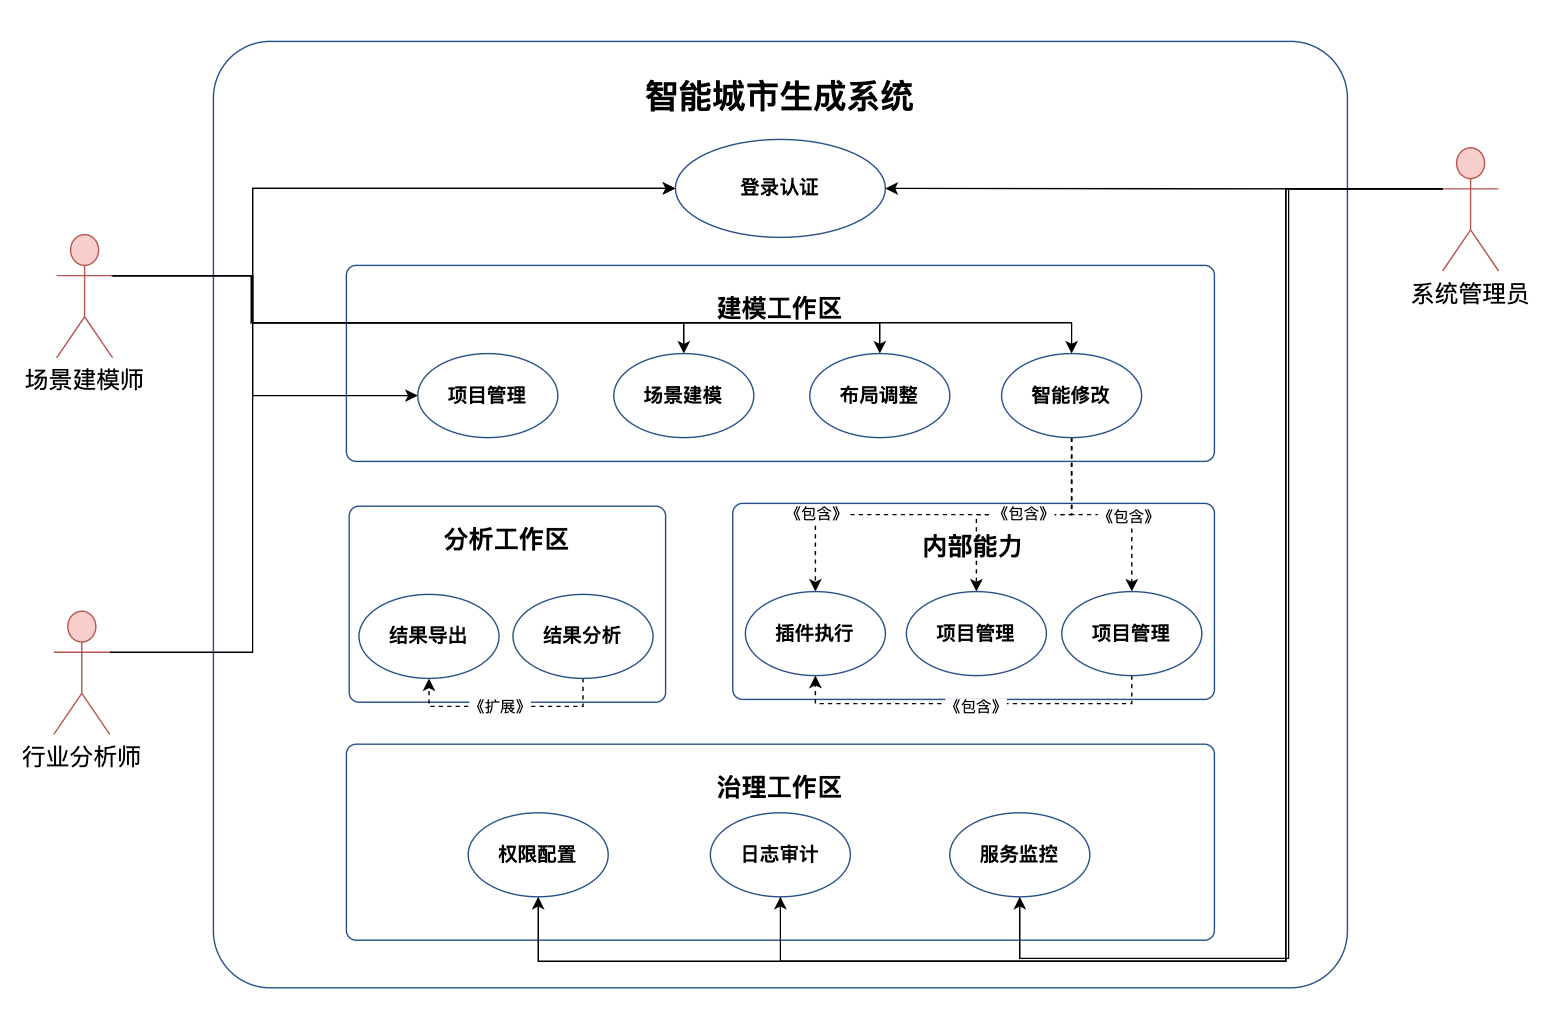
\includegraphics[width=\textwidth]{figures/01.png}
\caption{系统用例图}
\label{fig:oo_usecase}
\end{figure}

\subsection{类图}
图~\ref{fig:oo_class} 对系统静态结构进行了对象化展开，整体按身份与权限、项目与场景、任务与执行、仿真与治理四个对象域组织。身份与权限域由 \texttt{User}、\texttt{Role}、\texttt{Permission} 和 \texttt{Session} 组成，用于表达用户、角色、权限和会话之间的约束关系；项目与场景域由 \texttt{Project}、\texttt{SceneVersion}、\texttt{SceneObject}、\texttt{LayoutModel} 和 \texttt{Asset} 组成，用于表达项目聚合场景版本、场景版本承接布局与对象的组织方式；任务与执行域由 \texttt{TaskInput}、\texttt{ParseResult}、\texttt{StructuredCommand}、\texttt{Task}、\texttt{PluginJob} 和 \texttt{ExecutionResult} 组成，用于表达从输入规范化到任务执行结果回传的处理链路；仿真与治理域由 \texttt{SimulationPlan}、\texttt{DynamicObject} 和 \texttt{OperationLog} 组成，用于表达仿真结果和审计记录的承接关系。

在对象关系上，\texttt{Project} 聚合多个 \texttt{SceneVersion}，说明同一项目下允许保留多轮生成与修改结果；\texttt{SceneVersion} 聚合场景对象和布局模型，说明版本不仅保存最终对象集合，也保存其空间组织依据；\texttt{TaskInput} 与 \texttt{ParseResult}、\texttt{StructuredCommand}、\texttt{Task} 之间形成从输入理解到可执行命令的转换链；\texttt{Task} 进一步关联 \texttt{PluginJob} 和 \texttt{ExecutionResult}，说明系统内部将任务管理与插件执行结果显式区分；\texttt{SimulationPlan} 关联多个 \texttt{DynamicObject}，说明仿真方案负责承接动态交通、人群和船只等可观察对象；\texttt{OperationLog} 与用户和任务形成引用关系，说明关键操作和执行状态需要保留可追溯记录。

该图在设计上提供了三个静态基础。第一，项目、版本、任务和执行结果形成了系统的主数据骨架，使不同章节中的活动图、顺序图和状态图都可以围绕同一对象域展开。第二，解析结果与结构化命令的独立存在，说明 LLM 输出不会直接落到几何生成层，而是必须先转化为可验证、可调度的中间对象。第三，仿真对象、日志对象与核心任务对象并列存在，说明系统不仅关注生成，还同时关注结果分析与治理留痕。

\begin{figure}[!htbp]
\centering
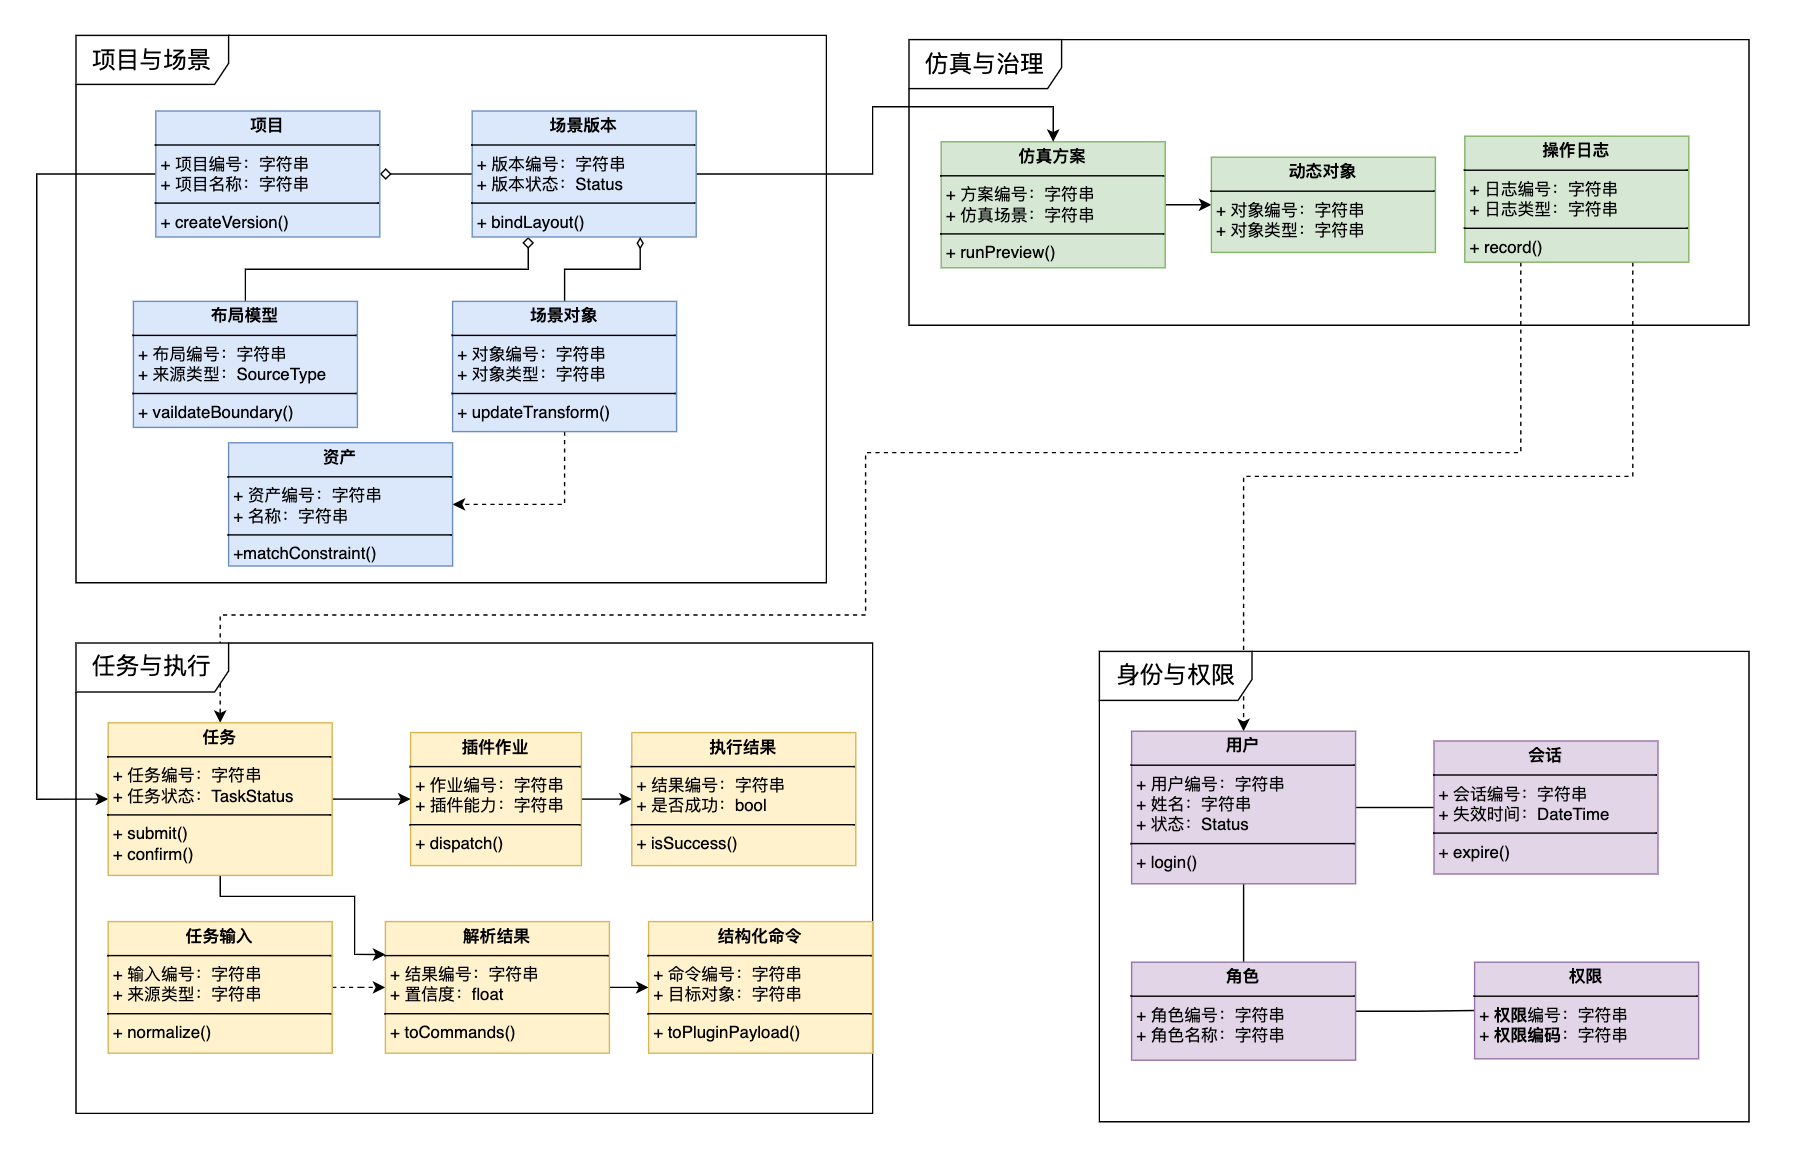
\includegraphics[width=\textwidth]{figures/02.png}
\caption{系统核心类图}
\label{fig:oo_class}
\end{figure}

\subsection{活动图}
活动图用于描述系统在控制流层面的组织方式。图~\ref{fig:oo_activity_main} 给出核心生成流程，图~\ref{fig:oo_activity_modeler}、图~\ref{fig:oo_activity_analyst} 和图~\ref{fig:oo_activity_admin} 分别补充三类角色在各自工作台中的活动路径。主活动图强调统一执行闭环，角色活动图强调不同用户在同一系统中的操作边界和回退路径。

\subsubsection*{1. 核心生成活动图}
核心生成活动图见图~\ref{fig:oo_activity_main}。流程从输入接收开始，依次经过场景上下文读取、意图解析、执行条件校验、任务确认、插件执行、版本保存和结果回看等环节。若当前输入无法直接执行，则流程返回补充信息和重新解析；若插件执行失败，则系统返回错误并允许重新提交；若结果仍需继续修改，则流程回到新的输入轮次。该图表达了系统以任务确认为界、以插件执行为核心、以版本回写和结果回看构成闭环的控制方式。

该图中的四个泳道分别对应场景建模师、主系统、LLM 解析模块和 Blender 插件，体现了控制权在不同处理阶段的转移方式。建模师负责提出意图和确认任务，主系统负责组织上下文、校验条件和登记状态，LLM 解析模块负责将输入转化为结构化任务建议，Blender 插件负责执行几何生成、替换或布局调整。这种泳道划分避免了将所有动作混写在单一流程中，使系统在控制层、解释层和执行层之间的职责边界更加清晰。

从控制逻辑上看，该图包含两个重要判定节点。第一个判定节点是“是否满足执行条件”，用于表达资源缺失、约束冲突或解析歧义时，流程必须回退到补充信息和重新解析，而不能直接进入执行。第二个判定节点是“执行是否成功”，用于表达插件执行后的失败重提与成功回写分流。结合最后的“是否继续修改”判断，该图完整刻画了系统从一次输入到多轮迭代的闭环机制。

\begin{figure}[!htbp]
\centering
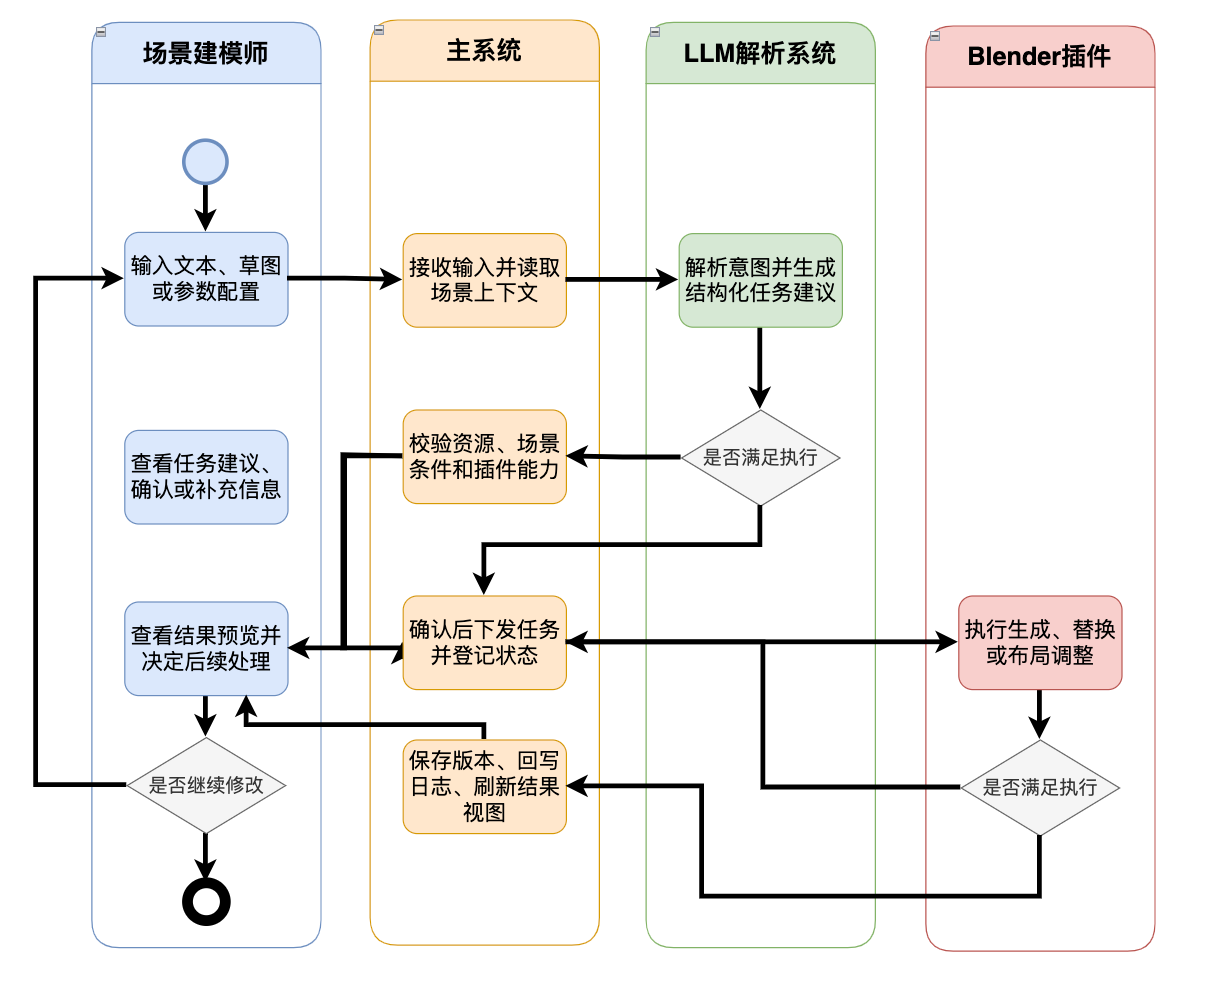
\includegraphics[width=\textwidth]{figures/04.png}
\caption{核心生成活动图}
\label{fig:oo_activity_main}
\end{figure}

\subsubsection*{2. 角色活动图}
图~\ref{fig:oo_activity_modeler} 进一步细化了场景建模师在建模工作台中的活动路径，覆盖项目选择、输入提交、任务确认、结果观察、版本保存与继续修改等环节，体现了多轮生成与局部修正过程。该图与主活动图相比，更强调建模师在版本创建、结果判断和局部重生成中的操作位置。

图中从“登录并进入建模工作台”开始，分化出“选择项目、创建版本或加载既有场景”和“输入文本、草图、点线集或参数配置”两条准备路径，随后在“查看解析后的任务建议并确认、补充或调整参数”处汇合，说明建模任务既依赖已有项目上下文，也依赖本轮输入内容。后续“观察生成结果与动态预览”以及“保存版本、导出场景或继续局部修改”构成结果处理阶段，其中判定节点“结果是否满足预期”决定流程是结束于版本保存，还是返回前部继续迭代。

该图支撑的设计重点在于说明建模师并非一次性提交后被动等待，而是持续参与项目版本组织、任务解释确认和结果质量判断三个环节。也就是说，系统中的智能建模并不是全自动批处理，而是一个带有人工确认和多轮反馈的交互式生产流程。

\begin{figure}[!htbp]
\centering
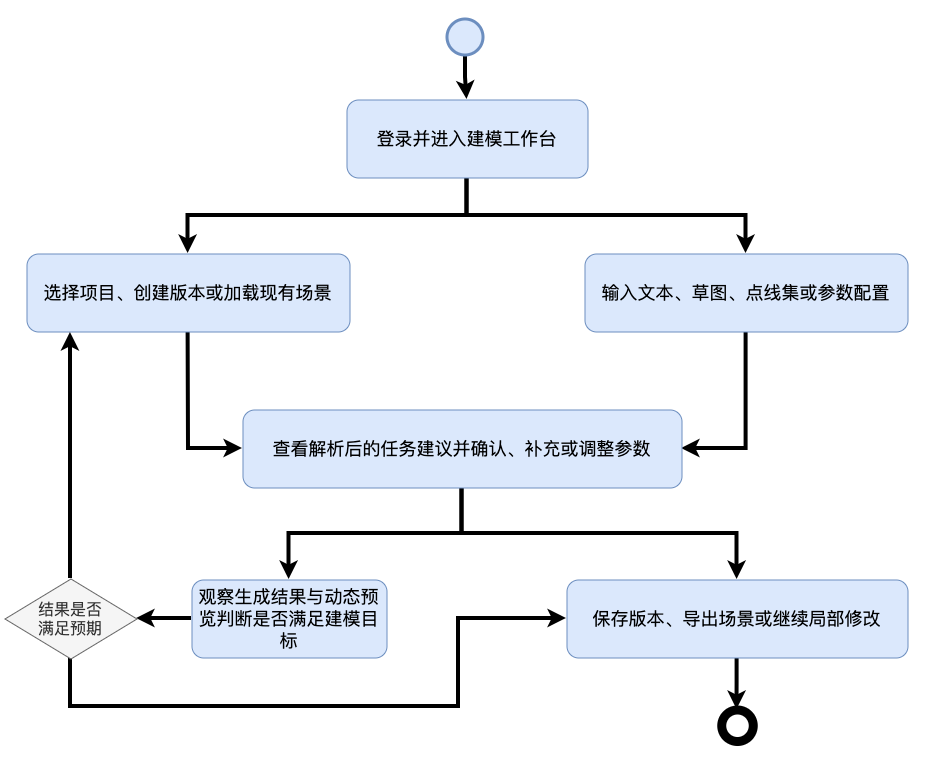
\includegraphics[width=0.9\textwidth]{figures/041.png}
\caption{场景建模师活动图}
\label{fig:oo_activity_modeler}
\end{figure}

行业分析师活动图对应图~\ref{fig:oo_activity_analyst}，其主线围绕分析对象选择、静态结果查看、仿真回放、方案比较和结果导出展开。该图反映了分析工作台以结果消费、仿真观察和多方案比较为主的处理链路。

图中先由分析师选择项目、方案或场景版本，确定待分析对象，再进入静态结果查看与关键指标查看阶段；之后通过“运行或回放仿真结果”观察车辆、人群、船只等动态差异，并在“比较不同方案并形成阶段性分析判断”节点形成分析结论。若仍需继续比较，则返回上游继续观察其他方案；若比较完成，则导出截图、结果文件或分析报告。

该图表明分析工作台并不承担生成职责，而是依赖已有版本和仿真结果开展消费、比较和判断工作。因此系统在这一角色下更强调结果可视化、指标一致性、对比链路和导出能力，而不是任务编排或插件执行能力。

\begin{figure}[!htbp]
\centering
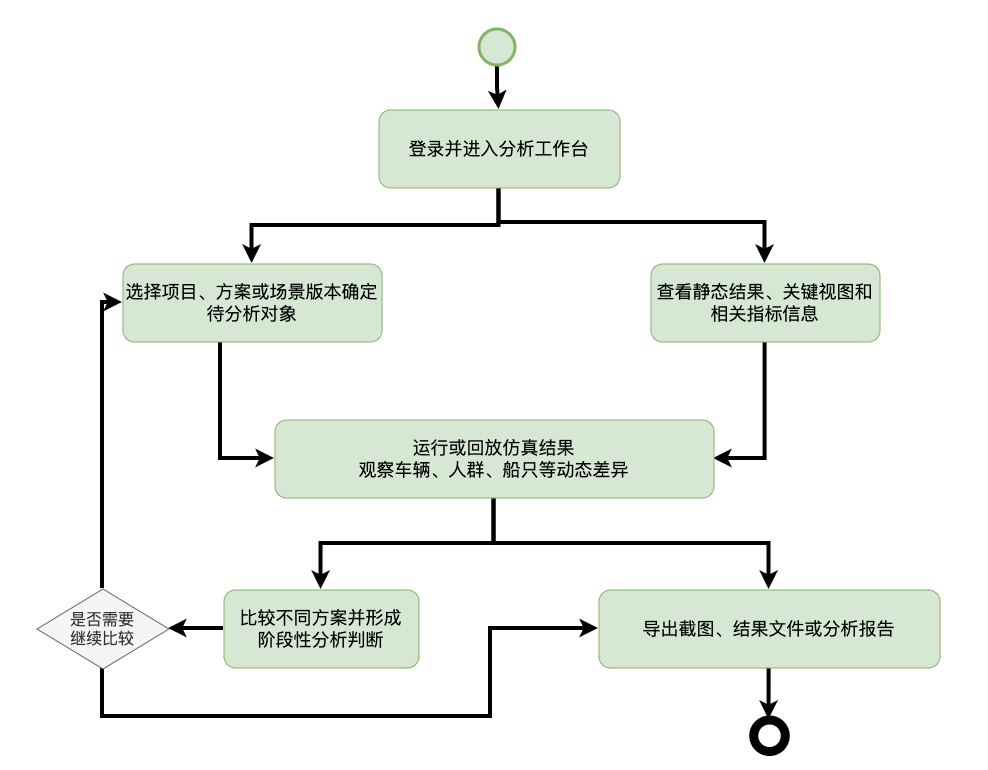
\includegraphics[width=0.9\textwidth]{figures/043.png}
\caption{行业分析师活动图}
\label{fig:oo_activity_analyst}
\end{figure}

系统管理员活动图如图~\ref{fig:oo_activity_admin}，围绕用户与权限维护、服务配置、任务监控、异常处理和审计留痕展开。该图表达了治理工作台以配置管理、运行监控和异常闭环处理为核心的维护过程。

图中从后台管理工作台进入后，分别展开为“维护用户、角色和权限关系”和“配置插件、模型服务和资源库接入状态”两类基础治理动作，随后汇合到“监控任务执行状态、查询日志并定位权限或服务异常”这一监控节点。若发现越权、失败任务或资源失效，则进入异常处理；若处理后仍存在持续异常，则流程回到上游继续巡检，否则通过“保存配置变更并形成审计记录”完成当前治理闭环。

该图所强调的不是业务产出，而是系统可用性和可追溯性。它说明管理员工作台必须同时支撑权限管理、服务接入、运行监控、异常处置和审计留痕五类能力，从而为建模和分析流程提供稳定的运行环境。

\begin{figure}[!htbp]
\centering
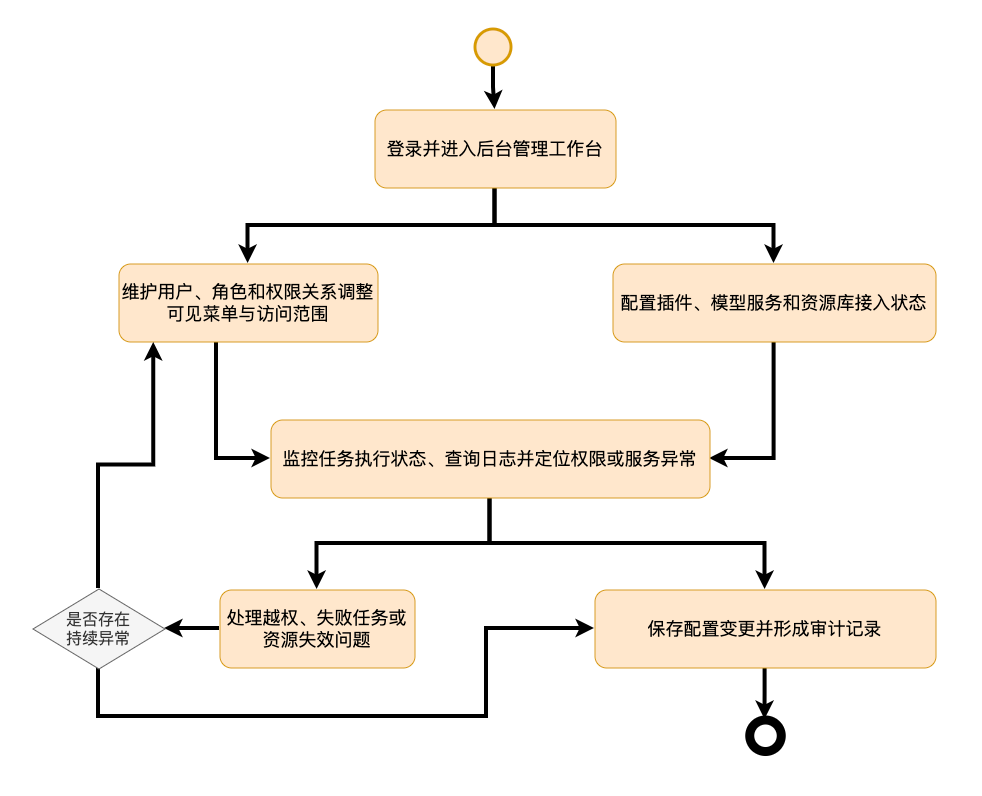
\includegraphics[width=0.9\textwidth]{figures/042.png}
\caption{系统管理员活动图}
\label{fig:oo_activity_admin}
\end{figure}

\subsection{顺序图}
顺序图~\ref{fig:oo_sequence} 按时间先后描述了一次建模任务的主要交互过程。建模师经由主系统提交输入后，任务编排模块先创建草稿并从项目存储读取上下文快照，再调用解析执行服务生成任务计划，并将任务解释返回界面。若当前信息不足，用户补充输入后重新进入解析；若任务可直接执行，则由用户确认后提交正式任务。随后，任务编排模块调用解析执行服务执行任务，在执行期间持续回传进度并更新界面状态，执行结束后完成版本保存和结果展示。

从参与对象上看，该图包含建模师、主系统、任务编排、解析执行服务和项目存储五个生命线。主系统负责接收输入并向编排层转交，任务编排负责承接草稿、组织上下文和控制后续流程，解析执行服务负责完成解析与执行，项目存储负责提供场景快照并保存最终结果。通过这种生命线划分，图中将“谁负责组织流程”和“谁负责执行业务”区别开来。

从消息序列上看，该图可以分为三个阶段。第一阶段是草稿创建与上下文读取，对应从 \texttt{submitInput()} 到 \texttt{loadContext()} 的调用链；第二阶段是任务解释与用户确认，对应 \texttt{parseIntent()}、\texttt{explainTask()}、\texttt{refineInput()} 和 \texttt{confirm()} 的交互；第三阶段是正式执行与结果回传，对应 \texttt{submitTask()}、\texttt{executeTask()}、\texttt{progress()}、\texttt{saveVersion()} 和 \texttt{showResult()}。该图明确了系统在时序上的职责分配和状态推进逻辑。

\begin{figure}[!htbp]
\centering
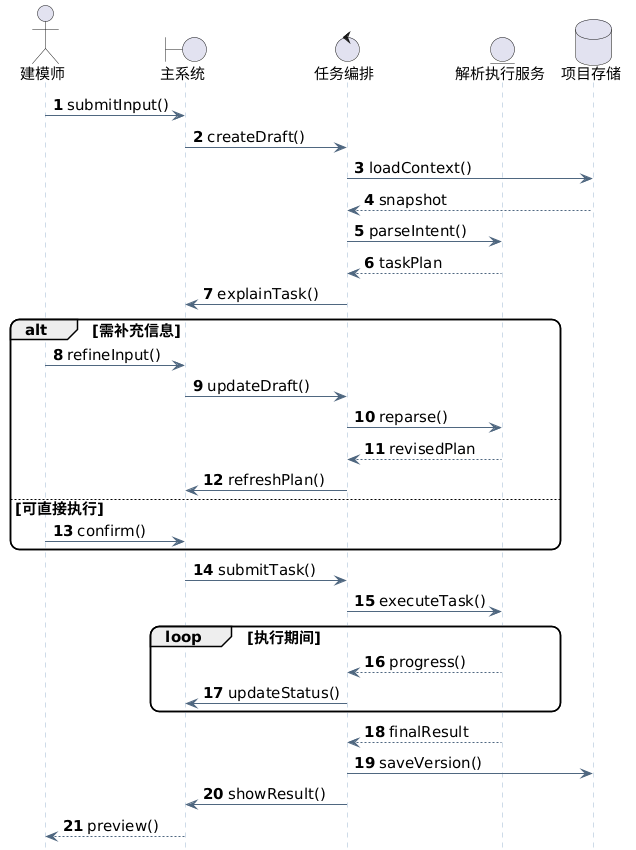
\includegraphics[width=\textwidth]{../UML_Project_Detailed_Fixed/03_SequenceDiagram.png}
\caption{场景任务顺序图}
\label{fig:oo_sequence}
\end{figure}

\subsection{协作图}
图~\ref{fig:oo_collaboration} 从对象协作角度展开了一次任务提交和执行过程，涉及建模工作台、任务编排器、资源上下文服务、LLM 解析服务、约束检查器、插件适配器、Blender 插件、版本管理器和仿真预览服务。任务编排器负责承接输入、读取上下文、调用解析和约束检查并返回任务解释；确认后，插件适配器负责下发插件作业，版本管理器负责生成新版本并请求仿真预览服务刷新结果。

与顺序图相比，该图更强调“哪些对象发生连接”和“消息如何在对象之间分发”。图中的任务编排器位于协作中心，一方面向资源上下文服务和 LLM 解析服务请求解释支持，另一方面向约束检查器获取告警和可执行性信息；确认后，消息通过插件适配器传递到 Blender 插件，再由版本管理器负责结果固化和面板刷新。仿真预览服务并不直接参与生成，而是在版本产生后提供可观察结果。

该图揭示了系统在对象协作层面的结构特点，即输入理解、约束校验、插件执行、版本管理和仿真预览并不是串成一个单体模块，而是通过一组相对独立的对象协同完成。这样的设计有利于后续替换解析服务、扩展插件能力或增补新的预览服务。

\begin{figure}[!htbp]
\centering
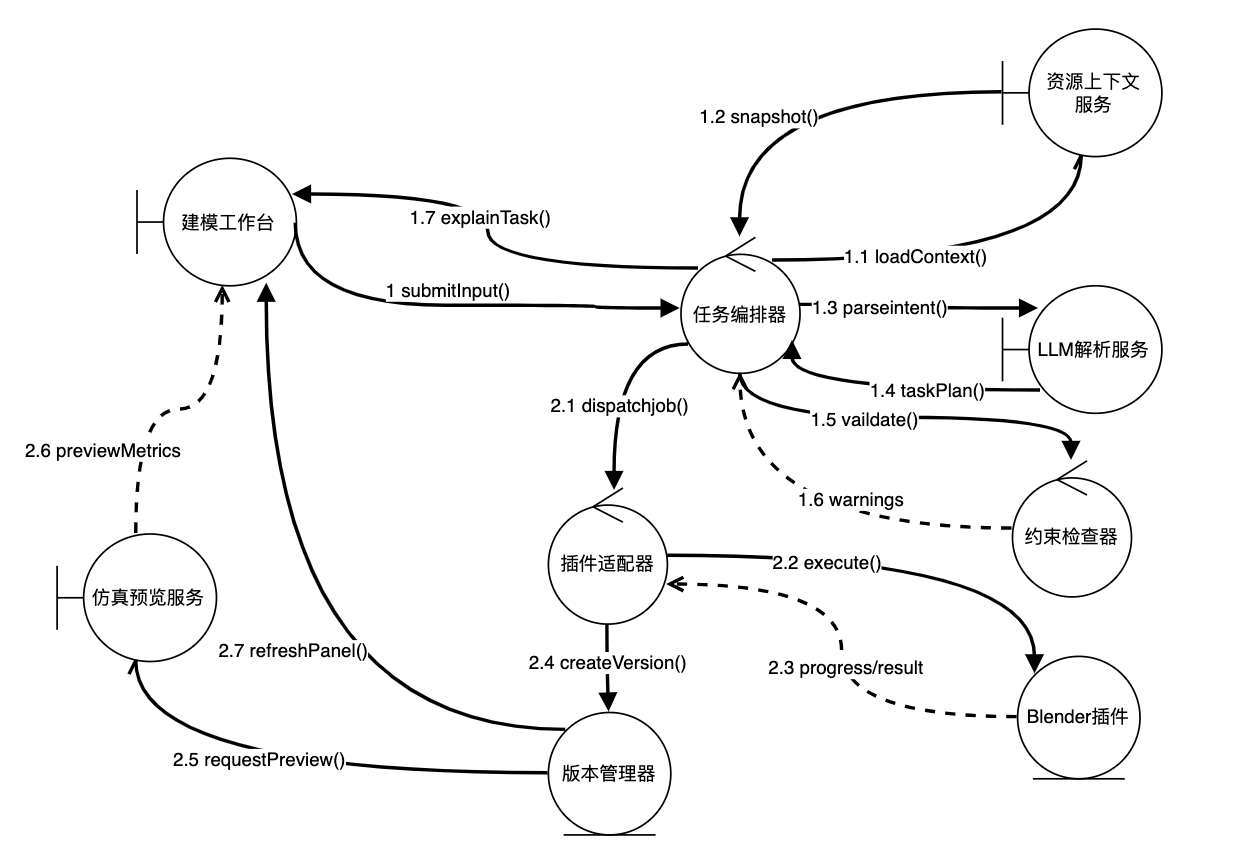
\includegraphics[width=\textwidth]{figures/05.png}
\caption{任务协作图}
\label{fig:oo_collaboration}
\end{figure}

\subsection{状态图}
状态图~\ref{fig:oo_state} 以 \texttt{Task} 为核心对象，描述任务从创建到归档的生命周期。任务创建后先处于草稿状态，提交解析后进入解析中；若存在歧义或条件缺失，则转入待补充，补充完成后重新解析；若生成结构化任务，则进入待确认；确认后进入排队中和执行中；执行成功后进入结果检查，再根据处理结果转入归档或回到草稿继续编辑；若解析或执行失败，则转入失败状态，并根据后续操作重新编辑或归档失败记录。

该图中的状态转换可以归纳为四个阶段。第一阶段是任务形成阶段，包括草稿、解析中和待补充，重点解决输入是否足以形成可执行任务的问题；第二阶段是任务确认阶段，由待确认状态承担，重点解决用户是否接受系统解释的问题；第三阶段是任务执行阶段，包括排队中和执行中，重点解决插件资源调度和执行反馈的问题；第四阶段是结果处理阶段，包括结果检查、失败、已取消和已归档，重点解决结果采纳、异常留痕和生命周期结束的问题。

状态图在设计上的意义在于将“任务是否存在”进一步细化为“任务当前处于何种处理位置”。这样一来，界面层可以基于状态决定允许的操作，调度层可以基于状态决定后续处理逻辑，日志层也可以基于状态变化形成清晰的审计轨迹。

\begin{figure}[!htbp]
\centering
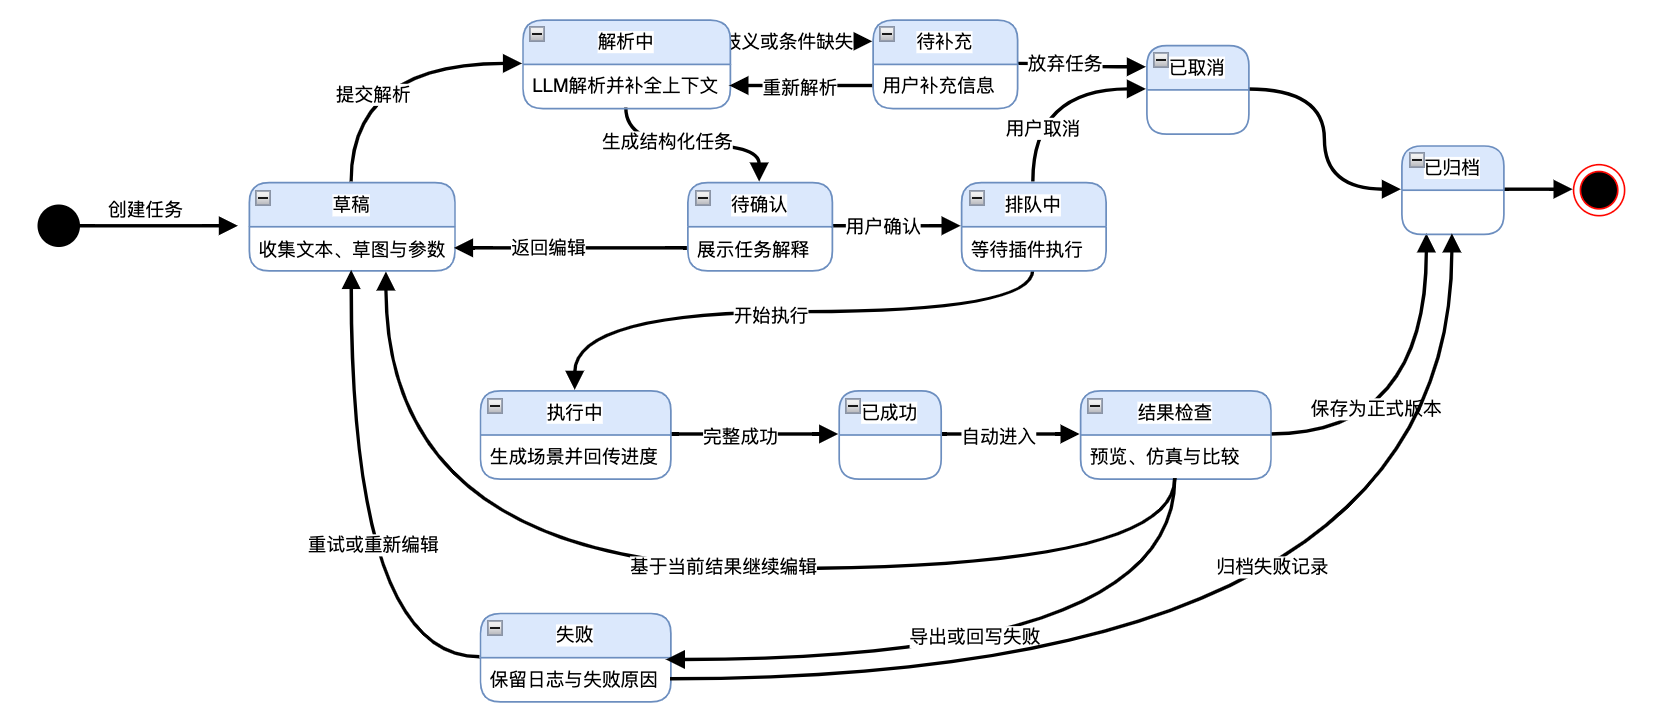
\includegraphics[width=\textwidth]{figures/06.png}
\caption{任务状态图}
\label{fig:oo_state}
\end{figure}

\subsection{构件图}
构件图~\ref{fig:oo_component} 给出了系统的软件构成单元及其依赖关系。主系统 UI 位于交互入口，任务调度服务位于核心控制位置，并分别依赖项目管理、权限、日志、LLM 接口适配和 Blender 插件适配等构件；Blender 插件适配器负责连接桌面端 Blender 插件；项目管理服务、日志服务和资源服务分别与数据库、文件存储和资产资源形成持久化依赖。

从构件分层上看，该图可以划分为交互层、服务层、执行层和基础设施层。交互层负责承接用户操作并展示结果；服务层负责项目管理、权限校验、任务调度、日志记录和资源访问；执行层负责连接 Blender 插件或外部模型服务；基础设施层负责数据库、文件和资产资源的持久化支撑。各层之间的依赖方向由上向下展开，避免交叉耦合。

该图的设计意义在于说明系统并不是以单进程方式实现所有功能，而是通过若干可替换、可扩展的构件协同工作。这样既便于隔离桌面端插件执行与服务端任务控制，也便于后续替换解析服务、调整存储实现或增加新的业务构件。

\begin{figure}[!htbp]
\centering
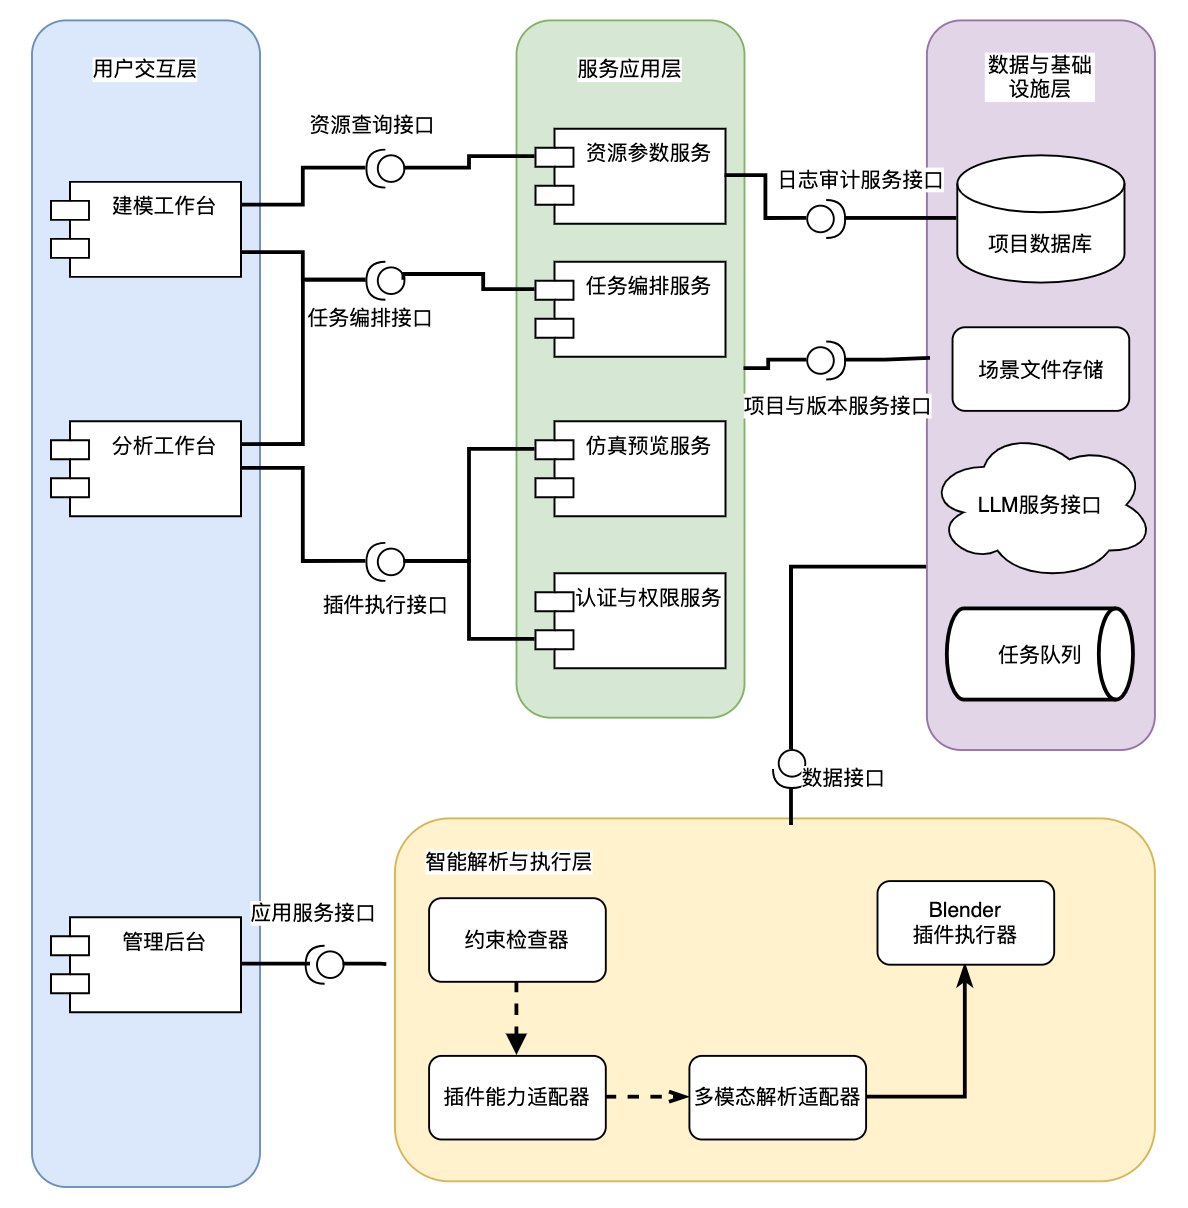
\includegraphics[width=\textwidth]{figures/07.png}
\caption{系统构件图}
\label{fig:oo_component}
\end{figure}

\subsection{部署图}
部署图~\ref{fig:oo_deployment} 描述了系统在运行环境中的节点划分与构件部署关系。用户工作站部署主系统前端界面、Blender 桌面端和城市生成插件；应用服务节点部署认证与权限服务、项目与版本服务、任务编排服务、资源参数服务、仿真预览服务和日志审计服务；模型服务节点部署 LLM 解析接口；数据与资源节点部署项目数据库、场景文件存储、资产资源库以及日志与备份目录。各节点之间通过登录鉴权、任务提交、解析请求、版本回写、资源读取和结果预览等通信链路相互连接，构成完整的运行环境。

从部署角色上看，用户工作站负责直接面向用户的交互与本地插件执行，应用服务节点负责业务控制与状态管理，模型服务节点负责解析能力输出，数据与资源节点负责持久化与资源供给。这样的部署划分使桌面执行环境、业务服务环境和模型推理环境相互分离，有利于分别扩展与维护。

从通信关系上看，前端界面既与应用服务节点交互，也通过任务编排服务间接驱动本地 Blender 插件；任务编排服务一方面向模型服务节点发起解析请求，另一方面向项目服务和日志服务写入上下文与执行结果；插件则直接访问场景文件存储和资产资源库完成本地生成与写盘。该图说明系统在运行层面采用“前端交互、本地执行、服务控制、集中存储”的协同方式。

\begin{figure}[!htbp]
\centering
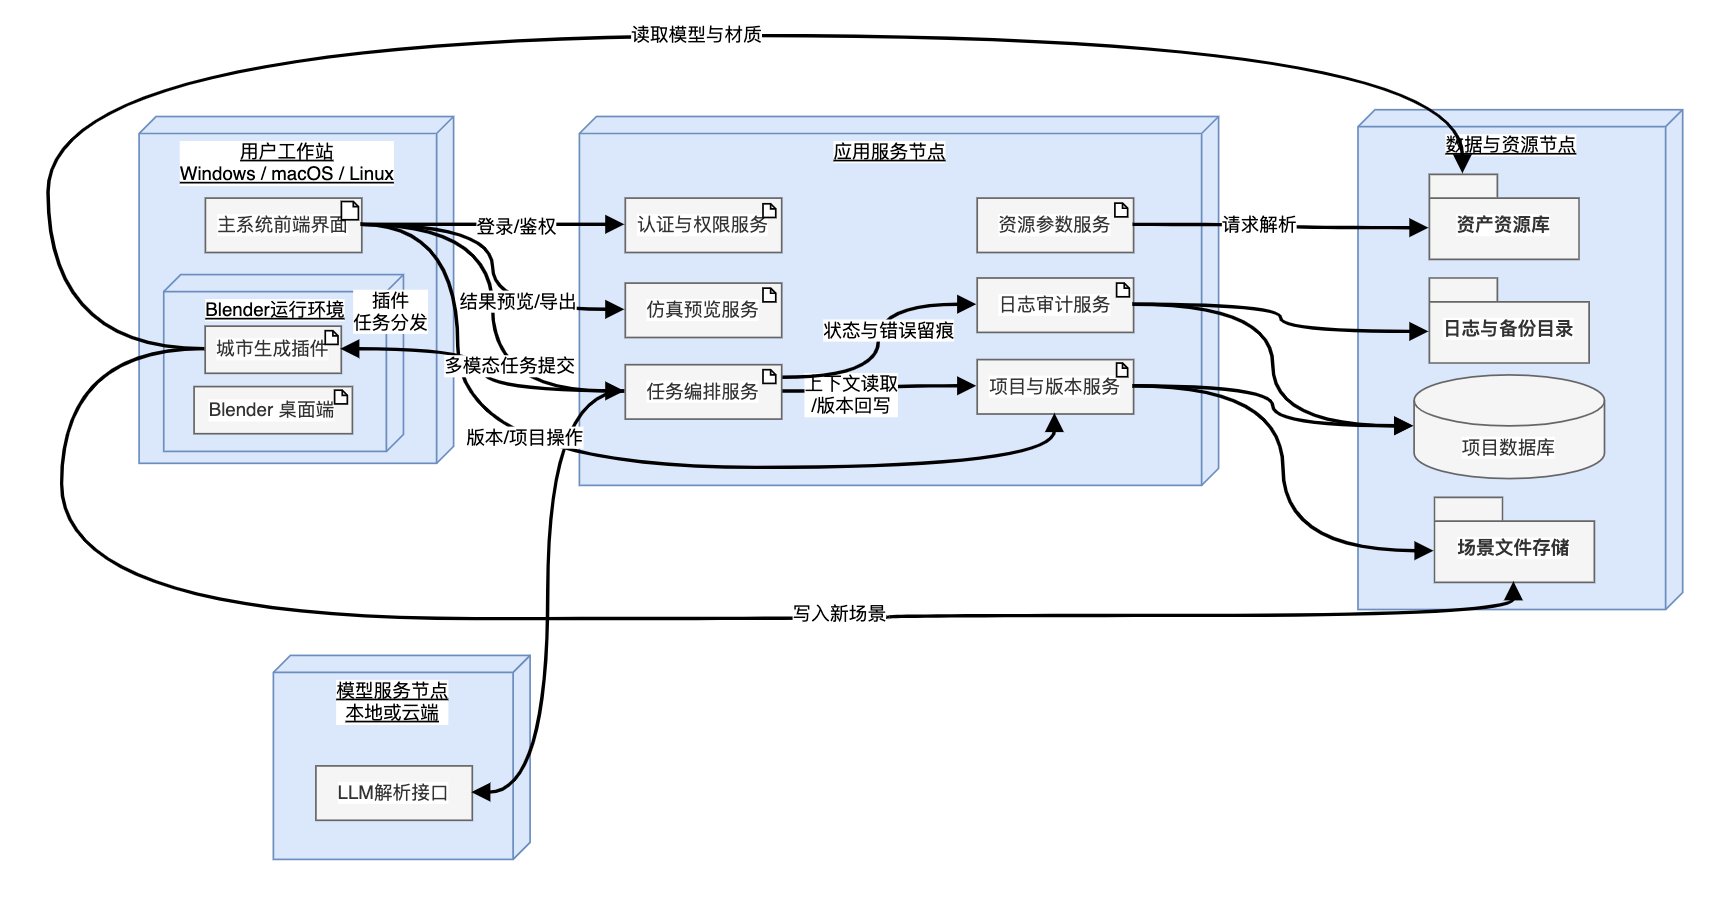
\includegraphics[width=\textwidth]{figures/08.png}
\caption{系统部署图}
\label{fig:oo_deployment}
\end{figure}

\subsection{统一命名与边界约定}
本章各类图在表达角度上各有侧重，但在命名和边界上保持一致。角色统一使用场景建模师、行业分析师和系统管理员；任务统一围绕 \texttt{Task}、\texttt{StructuredCommand}、\texttt{PluginJob} 和 \texttt{ExecutionResult} 组织；版本结果统一由 \texttt{SceneVersion} 承接；解析能力统一由 LLM 或解析执行服务承担；几何生成和场景落盘统一由 Blender 插件及其适配构件承担。这样的统一约定保证了各类图之间的语义连续性。

\section{界面设计}

\subsection{界面设计总览}
人机界面设计围绕角色分工和任务链路展开，整体采用统一登录入口与分角色工作台的组织方式。用户完成身份认证后，不同角色分别进入建模工作台、分析工作台和后台治理工作台。三类界面在导航位置、提示样式、状态反馈和日志入口上保持一致，以降低切换成本；在信息分区、操作入口和主视觉区域上则根据角色任务进行差异化设计。

从视觉层次上看，界面顶层均包含系统标题、当前项目或工作空间名称、角色标识、通知入口和个人菜单。左侧区域承担导航和对象切换功能，中部区域承担主要内容展示，右侧区域承担参数、属性、执行状态或明细信息展示。这样的布局既能够保持三类工作台在交互结构上的一致性，又能为不同角色提供有针对性的主操作区。

本章所述界面形态已结合生成的参考图进行整理。参考图为基于系统功能描述生成的设计示意，其作用在于辅助说明页面布局、视觉层次和信息分区，不作为最终实现界面或前端像素标准。报告中的界面描述以这些参考图所体现的结构关系为依据，并进一步将其转化为可实现的界面组织说明。

\subsection{登录入口界面}
登录入口界面采用简洁的双栏或单卡片结构。页面上方居中显示系统名称“智能城市生成系统”和简要说明文字，下方放置账号、密码和身份验证输入区，登录按钮位于表单底部居中位置。若采用双栏布局，左侧可展示城市场景示意图、系统能力摘要或三维城市缩略背景，右侧放置登录卡片；若采用单卡片布局，登录框位于页面中央，背景采用淡色城市网格、道路纹理或简化天际线图案。

该页面的重点是形成清晰的进入路径，而不是承载复杂信息，因此交互元素保持精简。除基础登录控件外，页面只保留“记住登录状态”“忘记密码”或“联系管理员”等辅助入口。登录失败时在表单附近以醒目的提示条显示错误信息；登录成功后根据用户角色自动跳转到对应工作台。

图~\ref{fig:ui_login_reference} 所示的登录页参考图采用左右分栏结构，左侧以城市天际线和河道道路场景作为主视觉背景，并叠加系统名称、能力口号和三项核心能力摘要；右侧为白色登录面板，包含语言切换、账号密码输入、记住我、找回密码、主登录按钮以及单点登录、微信登录等辅助入口。该图清楚表达了系统在视觉上兼顾“城市场景特征”和“企业软件入口”的设计方向，适合作为登录页的表现参考。

\begin{figure}[!htbp]
\centering
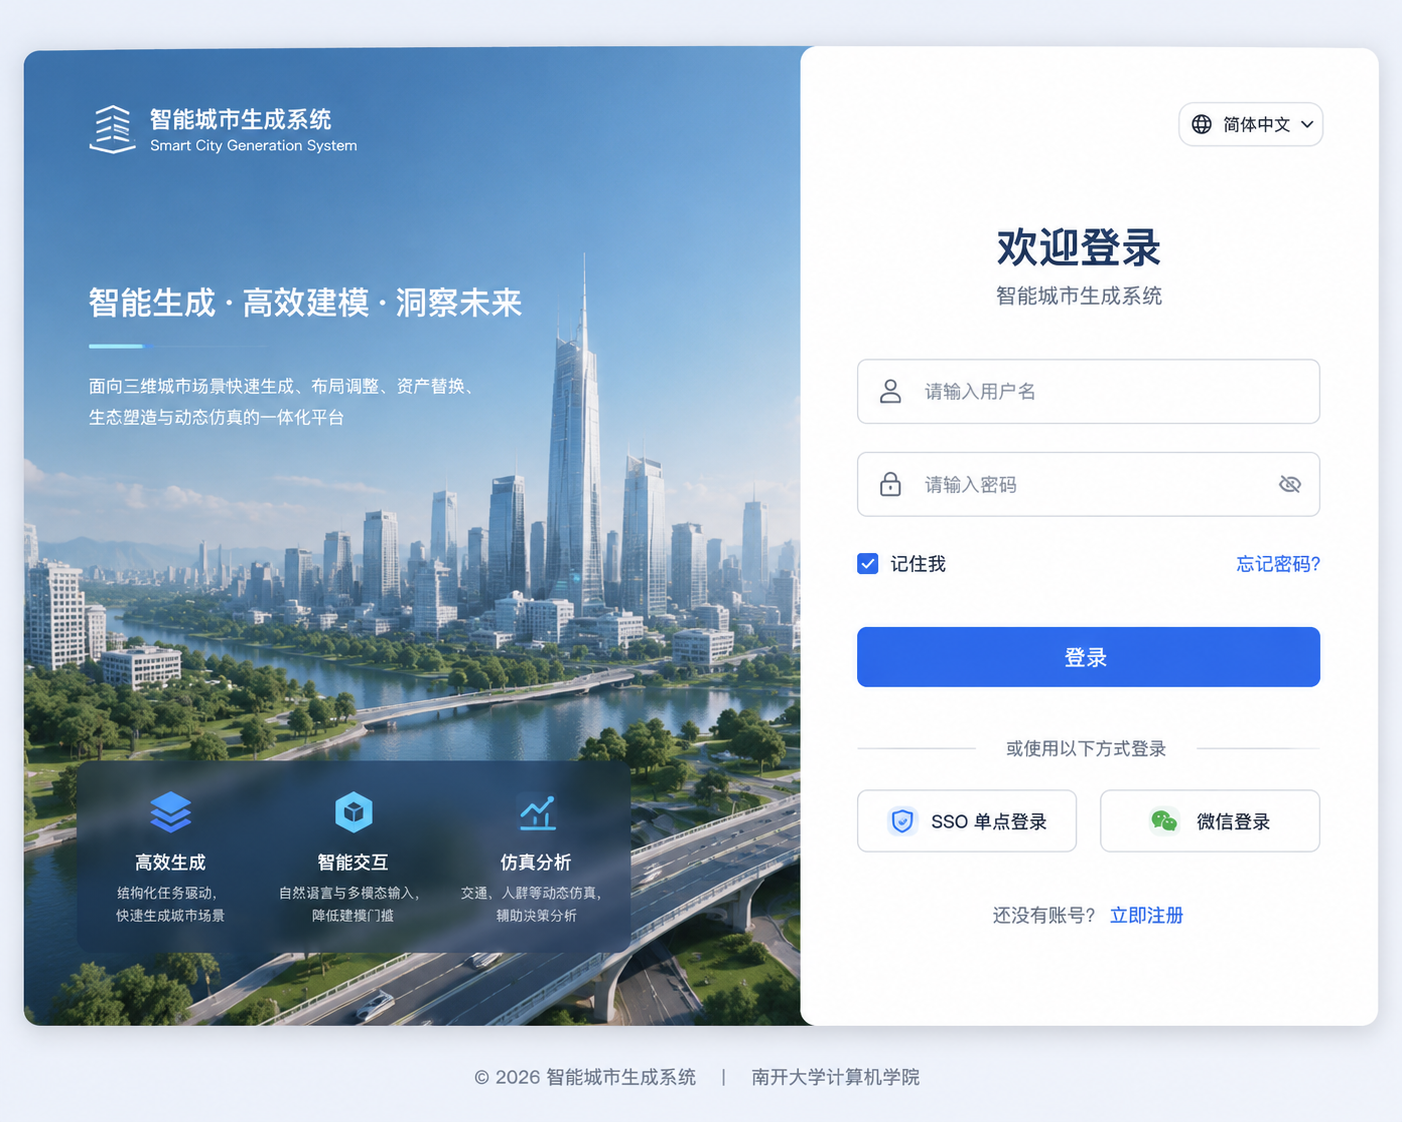
\includegraphics[width=\textwidth]{figures/11.png}
\caption{登录入口界面参考图}
\label{fig:ui_login_reference}
\end{figure}

\subsection{建模工作台}
建模工作台是系统的核心生产界面，整体采用三栏式结构。左栏用于项目与场景资源管理，顶部显示当前项目名称、版本号和最近保存时间，下方依次放置项目列表、场景版本树、资源分类标签以及可折叠的道路、建筑、植被、水体等资源面板。中部为主视图区，采用大尺寸三维场景预览窗口，可显示当前城市模型、控制点、布局轮廓和局部修改结果；主视图区下方放置时间轴、预览缩略条或版本对比切换入口。右栏为任务与参数区，按照“输入内容 - 结构化任务解释 - 参数确认 - 执行状态 - 结果摘要”的顺序自上而下排列。

在交互呈现上，建模师既可以通过文本输入框描述城市生成意图，也可以上传草图、点线集或参数模板。输入区下方显示系统生成的任务解释卡片，卡片内列出目标对象、数量、空间关系、限制条件和预计调用的插件能力。确认按钮、重新解析按钮和取消按钮位于任务卡片下方，执行后右栏切换为状态面板，显示排队中、执行中、成功或失败等状态标签、进度条和日志摘要。中部视图区在执行前后保持连续，便于建模师直接观察修改效果。

从界面氛围上看，建模工作台应突出“编辑中”的工作状态。中部三维视图占比最大，颜色以浅灰、蓝灰和少量强调色为主，资源列表和参数面板保持规整，执行按钮和异常提示使用高对比色进行区分。整体观感应接近专业设计软件或三维内容制作工具，而不是普通信息管理后台。

图~\ref{fig:ui_workbench_reference} 中的上左区域给出了建模工作台参考图，其结构与上述描述基本一致：左侧为导航与对象入口，中部为大尺寸三维城市视图，右侧为任务创建与任务状态区，下方额外保留任务队列表格。该设计强调“视图、任务、状态”三者在同一页面内联动，有利于支持文本输入、任务生成、结果观察和版本回看的连续操作。

\subsection{分析工作台}
分析工作台以结果查看、方案比较和仿真观察为中心，布局上可采用“左侧方案树 + 中央大视图 + 右侧指标面板”的结构。左栏显示项目、场景版本和分析方案列表，并支持切换不同时间片、不同策略或不同场景快照。中央区域是主要的结果展示窗口，可在静态城市视图、动态仿真回放视图和多方案分屏对比视图之间切换。右栏显示关键指标、统计图、筛选条件和导出入口，包括车辆密度、人流分布、船只流向、路网负载或区域热力强度等信息。

该界面不承担复杂建模编辑任务，因此输入控件明显少于建模工作台。顶部工具栏主要放置方案切换、回放控制、时间轴拖动、截图导出和报告生成按钮。中央主视图下方可配置仿真时间滑块、播放/暂停按钮和回放速度调节控件，用于观察动态变化。若采用双方案比较模式，中央区域可左右并排显示两个方案视图，中间保留同步滚动或联动回放开关。

在视觉表达上，分析工作台强调“观察”和“比较”。地图、三维场景、热力叠加层和动态图例构成主要视觉元素，图表和统计卡片辅助解释结果。界面应弱化资源库、参数编辑器和插件配置等生产型控件，使分析师能够将注意力集中在结果差异和指标变化上。

图~\ref{fig:ui_workbench_reference} 的上右区域展示了分析工作台参考图。该图采用热力覆盖与指标卡片并置的方式：中央显示带有交通与区域热力叠加效果的城市视图，右侧展示人口、交通、能耗等指标摘要及趋势图，下方提供图层控制和仿真对象筛选区。该布局较好地体现了分析界面对“结果读取、指标解释、方案对比”的侧重关系。

\subsection{管理员工作台}
管理员工作台采用信息管理后台样式，整体结构为“左侧功能导航 + 中央列表区域 + 右侧详情抽屉或下方详情面板”。左侧导航包含用户管理、角色权限、插件连接、模型服务、资源库状态、任务监控、日志审计和系统配置等模块。中央区域默认显示表格或卡片列表，支持搜索、筛选、排序和批量操作。右侧详情区在点击某一记录后展开，用于显示用户权限矩阵、插件状态明细、服务健康信息、错误日志片段或审计追踪记录。

管理员界面中的任务监控页应突出运行状态面板，上方放置服务健康概览卡片，例如“在线插件数”“任务排队数”“近一小时失败率”“模型服务响应时间”等摘要信息；下方显示任务列表和日志表格，每条记录包含任务编号、触发用户、当前状态、开始时间、结束时间和异常说明。权限管理页则更强调角色树、菜单矩阵和权限勾选区，以便管理员快速调整可见功能和操作范围。

该工作台在视觉上应保持克制和清晰。颜色以中性色为主，异常状态使用橙色或红色强调，成功状态使用绿色标识。界面重点在于信息可检索、状态可定位、操作可追溯，不需要突出三维效果或沉浸式展示。

图~\ref{fig:ui_workbench_reference} 的下方区域给出了管理员工作台参考图。该图采用典型后台布局，上方为系统概览卡片，中部为趋势图与资源监控图，下方为项目存储使用情况、系统服务状态和最近日志列表。该图将管理员最关心的统计信息、运行状态和审计记录集中在同一页面上，适合作为后台首页或综合监控页的设计参考。

\begin{figure}[!htbp]
\centering
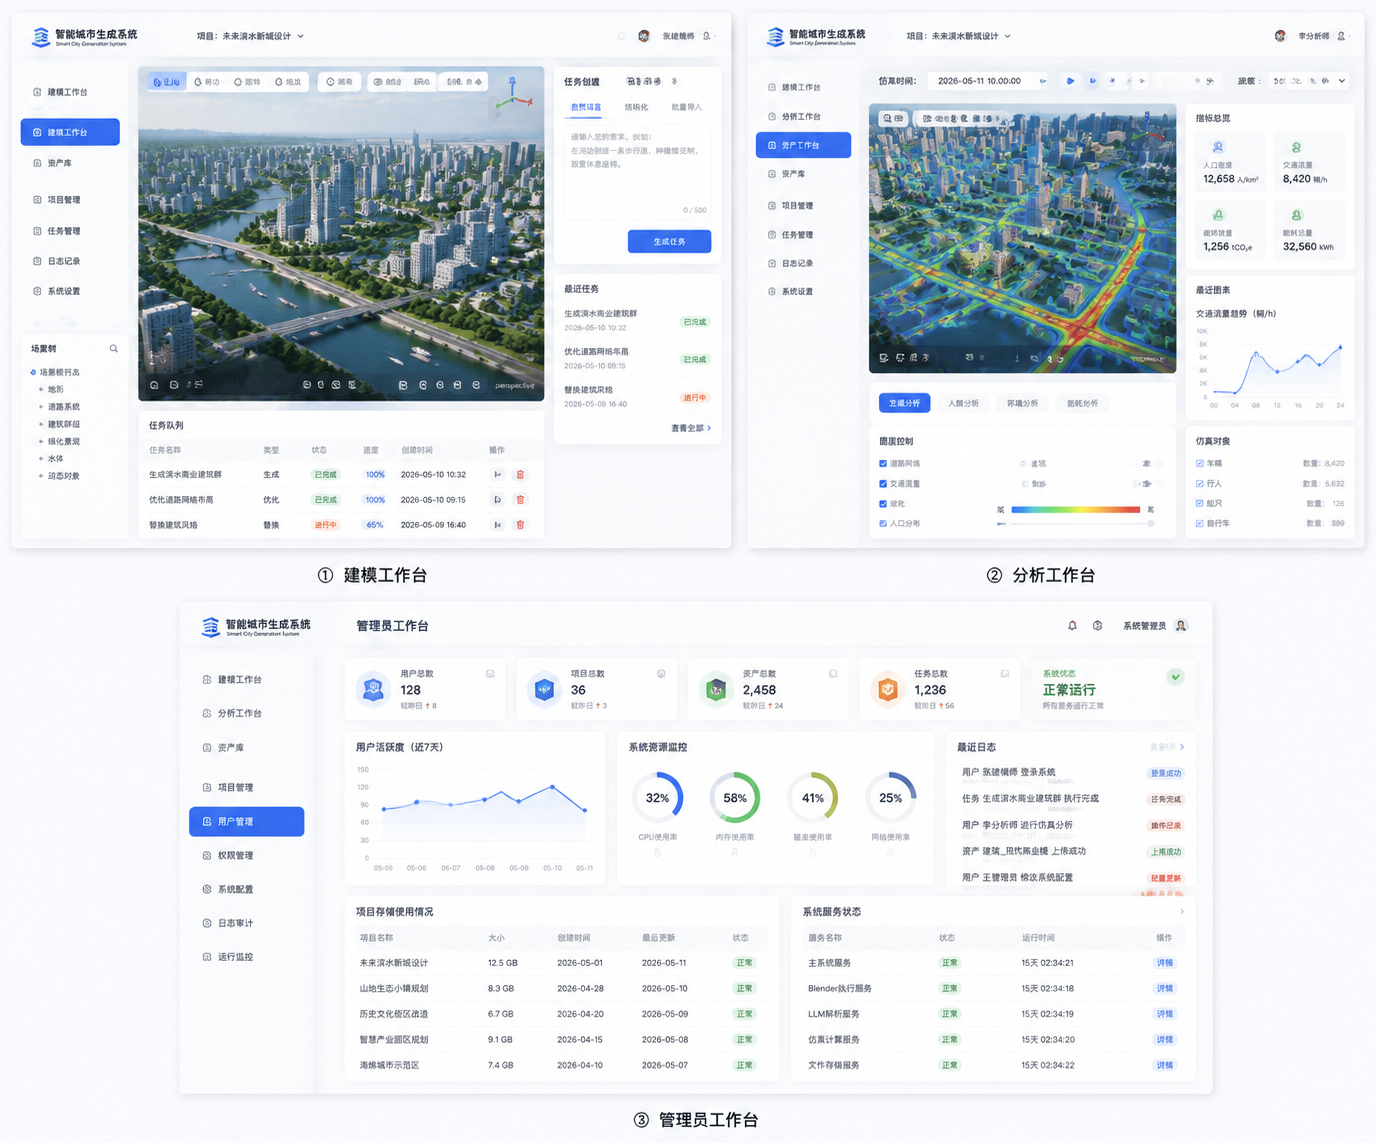
\includegraphics[width=\textwidth]{figures/12.png}
\caption{三类工作台界面参考图}
\label{fig:ui_workbench_reference}
\end{figure}

\subsection{界面设计原则}
\begin{enumerate}[label=\arabic*.]
    \item 执行前信息可解释：建模相关界面必须在任务下发前显示结构化解释、约束条件和关键参数。
    \item 状态反馈持续可见：排队、执行、成功、失败和回写等状态均需在显著位置连续显示。
    \item 角色入口保持收敛：每类角色仅暴露完成本职任务所需的主要功能和信息面板。
    \item 结果与版本易于回看：项目版本、仿真结果、日志摘要和导出入口应能快速定位。
    \item 主操作区视觉突出：建模工作台突出三维视图，分析工作台突出结果对比，管理员工作台突出列表与状态面板。
\end{enumerate}

\section{总结}
本文围绕智能城市生成系统的软件设计展开说明，从系统概述、架构分解、数据组织、面向对象建模和界面设计五个层面给出了较为完整的设计描述。报告明确了主系统、Blender 插件执行端、解析服务、仿真服务以及数据与资源存储之间的职责边界，也对项目、场景版本、任务、结构化命令、插件作业、执行结果和日志等核心对象进行了统一组织。

从体系结构上看，系统采用任务驱动的组织方式：用户输入首先在主系统中完成接收、解释和确认，再由任务编排机制驱动插件执行与结果回写；从数据设计上看，系统以项目、版本和任务为主线，以仿真对象和操作日志作为辅助支撑，从而满足结果回看、版本比较和过程追溯的需要；从面向对象设计上看，报告通过用例图、类图、活动图、顺序图、协作图、状态图、构件图和部署图对系统的静态结构、动态行为、软件构成和运行环境进行了系统化表达；从界面设计上看，系统以统一登录入口和分角色工作台为交互基础，使建模、分析和治理三类活动能够在一致的导航逻辑下完成。

综合而言，本报告所描述的软件设计方案体现了三个核心特征：其一，以结构化任务作为自然语言输入与几何生成执行之间的中间桥梁，从而控制解析结果的可解释性与可执行性；其二，以场景版本和任务状态管理为基础，实现生成、修改、分析和归档过程的连续衔接；其三，以角色分工和构件分层为原则，使交互层、控制层、执行层和存储层之间保持清晰边界。上述设计为系统后续实现、接口细化、模块协同和运行部署提供了统一依据。


\end{document}
